\documentclass{exam_template}

\usepackage{arydshln}

\usepackage{minted}
\usemintedstyle{friendly}
\setminted{fontsize=\small}
\renewcommand{\ttdefault}{cmtt}

\title{\bfseries Залікова робота \\з предмету <<Прикладні \\ задачі аналізу великих даних>>}
\author{\bfseries Захаров Дмитро, Варіант 5}
\date{31 травня, 2025}

\begin{document}

\pagestyle{fancy}

\maketitle

\tableofcontents

\newpage

\section{Задача 1}

\begin{problem}
    Що включає описова статистика? Як ці показники пов’язані між собою і про що
говорять? \textit{(15 балів).}
\end{problem}

\subsection{Загальне означення}\label{sec:descriptive_statistics}

\begin{definition}
\textbf{Описова статистика} це сукупність методів, які
використовуються для систематизації та представлення даних у вигляді графіків і
таблиць, а також числовим узагальненням за допомогою ключових статистичних
показників.
\end{definition}

Помітимо, що вона не робить жодних висновків про генеральну сукупність, а лише
описує наявні дані. Зазвичай, використовуються наступні три методи 
агрерування та представлення даних:
\begin{itemize}
    \item \textbf{Графічні методи} — це діаграми, гістограми, графіки та інші
    візуальні представлення даних.
    \item \textbf{Табличні методи} — рядки і стовпці, в якій в певному порядку
    викладається певна статистична інформація про задані події чи процеси.
    \item \textbf{Статистичні показники} — це числові характеристики, які
    узагальнюють дані, наприклад, середнє значення, медіана, мода, дисперсія
    (будемо розглядати більш детально надалі).
\end{itemize}

\subsection{Методи середнього рівня}\label{sec:central_tendency}
Які саме статистичні показники використовуються? Розглянемо основні 
методи середнього рівня, що усереднюють певні показники даних.

\subsubsection{Середнє значення}\label{sec:mean}
Якщо вважати вибірку даних $X_1,\dots, X_n \sim X$ елементами, що розподілені
незалежно однаково за певним розподілом $X$ (на практиці, неперервним з густиною
$\rho_X$), то нас може цікавити, наприклад, середнє значення цих даних. Для
цього, в теорії ймовірностей, ми використовуємо \textbf{математичне сподівання},
яке в загальному випадку для величини $X$ з кумулятивною функцією розподілу
$F_X$ над ймовірнісним простором $\Omega$ визначається як $\mathbb{E}[X]
\triangleq \int_{\Omega} x dF_X(x)$. Незміщенною та асимптотично стійкою оцінкою
математичного сподівання розподілу є \textit{вибіркове середнє} $\overline{X}
\triangleq \frac{1}{n}\sum_{i=1}^n X_i$, тобто це означає, що
$\mathbb{E}[\overline{X}] = \mu$ та $\overline{X} \xrightarrow{}
\mu$\footnote{Якщо ще більш формально, то $\forall \varepsilon > 0: \lim_{n \to
\infty}\text{Pr}\left[\left|\overline{X}_n - \mathbb{E}[X]\right| >
\varepsilon\right] = 0$, де $\overline{X}_n \triangleq \frac{1}{n}\sum_{i=1}^n
X_i$.}, де $\mu$ — математичне сподівання розподілу $X$. Проте, у випадках, коли
структура даних або природа задачі вимагає врахування певних особливостей, ми
можемо використовувати і інші види середнього значення:
\begin{itemize}
    \item \textcolor{blue!70!black}{Гармонійне середнє} визначається як
    $\overline{X}_H \triangleq \frac{n}{\sum_{i=1}^n X_i^{-1}}$ і
    використовується, коли дані представляють собою швидкості або інші величини,
    що мають зворотну пропорційність. Наприклад, якщо ви їдете $n$ відстаней
    $\ell$ з різними швидкостями $v_i$, то середня швидкість $\overline{v} =
    \frac{\ell}{T}$, де $T = \sum_{i=1}^n \frac{\ell}{v_i}$, буде дорівнювати
    саме гармонійному середньому $\overline{v}_H$. Також її можна зустріти для 
    обрахунку метрики $F_1$-score в задачах класифікації, де вона використовується
    для обчислення середньої гармонійної точності та повноти (precision та
    recall).
    \item \textcolor{blue!70!black}{Геометричне середнє} визначається як
    $\overline{X}_G \triangleq \left(\prod_{i=1}^n X_i\right)^{1/n}$ і
    застосовується для даних, що мають відношення до відсотків або відносних
    змін.
    \item \textcolor{blue!70!black}{Квадратичне середнє} визначається як
    $\overline{X}_Q \triangleq \sqrt{\frac{1}{n} \sum_{i=1}^n X_i^2}$ і
    використовується для даних, що мають відношення до енергії та потенціалу
    (наприклад, в електриці або механіці). Також, саме це середнє часто
    використовується в машинному навчанні для оцінки якості моделей, наприклад,
    в середньоквадратичній помилці (MSE).
    \item \textcolor{blue!70!black}{Степеневе середнє} визначається як
    $\overline{X}_p \triangleq \left(\frac{1}{n} \sum_{i=1}^n X_i^p
    \right)^{1/p}$, де $p$ — це параметр, що визначає ступінь середнього.
    \item \textcolor{blue!70!black}{Взважене середнє}: якщо кожному елементу
    вибірки $X_i$ відповідає вага $w_i$ (причому, без обмеження загальності,
    нехай $\sum_{i=1}^n w_i = 1$), то взагальне середнє визначається як
    $\overline{X}_W \triangleq \sum_{i=1}^n w_i X_i$. Це середнє
    використовується, коли дані мають різну важливість або, наприклад, мають
    різну точність. Зокрема, якщо ми знаємо дисперсію кожного показника $X_i$,
    то можна задати $w_i \propto \frac{1}{\text{Var}[X_i]+\varepsilon^2}$ для
    малого $\varepsilon$.
\end{itemize}

\subsubsection{Медіана та мода}\label{sec:median_mode}

Окрім середніх значень, для опису середнього рівня часто використовуються
\textbf{медіана} та \textbf{мода}. Медіана визначається як значення, яке
розділяє вибірку даних на дві рівні частини, тобто половина значень менша або
дорівнює медіані, а інша половина більша або дорівнює їй. Показує центральне
розташування даних і менш чутлива до викидів і асиметрії, ніж середнє. Більш
формально, для величини $X$, медіаною називаємо таке значення $M$, для якого
$F_X(M) = \text{Pr}[X \leq M] = 0.5$. В свою чергу модою $M_0$ називаємо таке
значення, яке має найбільшу ймовірність в розподілі $X$, тобто $M_0 =
\arg\max_{\omega \in \Omega} \rho_X(\omega)$ для густини розподілу $\rho_X$.
Згідно означенню, показує, яке значення найчастіше зустрічається в даних.
Особливо корисна для категоріальних даних або даних з дискретним розподілом. 

\subsection{Методи розсіювання (варіабельність)}\label{sec:dispersion_methods}

\subsubsection{Дисперсія, стандартне відхилення}\label{sec:dispersion}
До методів розсіювання відносяться статистичні показники, які
вимірюють, наскільки дані розкидані навколо середнього значення. Це важливо
для розуміння того, наскільки дані варіюються --- наприклад, для 
визначення точності вимірювань або для оцінки ризиків в фінансових
операціях.

Перша, найпростіша та найпоширеніша міра розсіювання — це \textbf{дисперсія},
яка визначена як $\text{Var}[X] = \mathbb{E}[(X-\mathbb{E}[X])^2]$ --- тобто
буквально середнє квадратичне відхилення від середнього значення. У вигляді
інтегралу для неперервного розподілу вона виглядає як $\text{Var}[X] =
\int_{\Omega} (x-\mathbb{E}[X])^2dF_X$. Дуже часто використовується
\textbf{стандартне відхилення}, яке визначається як $\sigma_X =
\sqrt{\text{Var}[X]}$, що дозволяє зберегти одиниці виміру та зробити іноді
інтерпретацію більш зрозумілою: наприклад, якщо ми маємо дані про висоту людей,
то дисперсія буде мати розмірність $m^2$, в той час як стандартне відхилення
буде просто в метрах, що більш інтуїтивно. Геометрично ми проілюструємо ці
поняття на прикладі нормального розподілу: див.
Рисунок~\ref{fig:normal_distributions}.

\begin{figure}[H]
\centering
\begin{tikzpicture}
\begin{axis}[
    domain=-8:8,
    samples=200,
    axis lines=middle,
    xlabel={$x$},
    ylabel={$\mathcal{N}(x;\mu,\textcolor{blue}{\sigma})=\frac{1}{\sqrt{2\pi}\textcolor{blue}{\sigma}}\exp\left(-\frac{(x-\mu)^2}{2\textcolor{blue}{\sigma}^2}\right)$},
    legend style={at={(1.05,0.5)}, anchor=north west},
    title={\textcolor{blue!80!black}{\textbf{Нормальний розподіл з різними дисперсіями $\sigma^2$}}},
    height=8cm, width=12cm,
    grid=both,
    ultra thick,
    ymin=-0.1, ymax=0.7,
]

% Normal distribution with variance = 0.5
\addplot [blue] {1/sqrt(2*pi*0.5) * exp(-x^2/(2*0.5))};
\addlegendentry{$\sigma^2 = 0.5, \mu=0$}

% Normal distribution with variance = 1
\addplot [red] {1/sqrt(2*pi*1) * exp(-x^2/(2*1))};
\addlegendentry{$\sigma^2 = 1, \mu=0$}

% Normal distribution with variance = 2
\addplot [green!60!black] {1/sqrt(2*pi*2) * exp(-x^2/(2*2))};
\addlegendentry{$\sigma^2 = 2, \mu=0$}

% Normal distribution with variance = 4
\addplot [orange] {1/sqrt(2*pi*4) * exp(-x^2/(2*4))};
\addlegendentry{$\sigma^2 = 4, \mu=0$}

\end{axis}
\end{tikzpicture}
\caption{Нормальні розподіли $\mathcal{N}(x;\mu,\sigma^2)$ з різними дисперсіями
$\sigma^2$ та нульовим математичним сподіванням $\mu=0$. Як бачимо, чим більша 
дисперсія, тим ширше розподілені дані навколо середнього значення.}
\label{fig:normal_distributions}
\end{figure}

Щоб обрахувати дисперсію вибірки даних $X_1,\dots, X_n$, ми можемо
використовувати \textit{вибіркову дисперсію}, яка визначається як
\begin{equation*}
    \widehat{\sigma}^2 \triangleq \frac{1}{n-1} \sum_{i=1}^n (X_i - \overline{X})^2,
\end{equation*}

Ця оцінка є незміщеною, тобто $\mathbb{E}[\widehat{\sigma}^2] =
\text{Var}[X]$, і асимптотично стійкою, тобто $\widehat{\sigma}^2
\xrightarrow{\rho} \text{Var}[X]$ при $n \to \infty$. Вона використовується
для оцінки дисперсії генеральної сукупності на основі вибірки даних.

\subsubsection{Стандартна помилка}\label{sec:standard_error}

Термін був вперше введений в 1897 році Удні Юлом і визначений для розподілу з
дисперсією $\sigma^2$ як $\text{SD}(\mu) \triangleq \frac{\sigma}{\sqrt{n}}$.
Проте, оскільки ми ніколи не знаємо дисперсію генеральної сукупності, то ми
використовуємо $\text{SE}(\overline{X}) \triangleq
\frac{\widehat{\sigma}}{\sqrt{n}}$. Цей показник береться з центральної
граничної теореми, яка стверджує, що при достатньо великому розмірі вибірки $n$
розподіл вибіркового середнього $\overline{X}$ буде наближатися до нормального
розподілу $\mathcal{N}\left(\mu,\frac{\sigma^2}{n}\right)$, де як раз таки
$\frac{\sigma^2}{n}$ є дисперсією вибіркового середнього. Далі цей параметр може
бути використаний для побудови довірчих інтервалів, перевірки гіпотез
(наприклад, $z$-тести/$t$-тести) тощо.

\subsubsection{Коефіцієнт ексцесу (Kurtosis) та асиметрії (Skewness)}\label{sec:kurtosis_skewness}

\textbf{Коефіцієнт ексцесу} $\kappa[X]$ показує ``крутість'' підвищення кривої
розподілу $X$ відносно нормального розподілу. Він визначається як момент
четвертого порядку стандартної величини $Z =
\frac{X-\mathbb{E}[X]}{\sqrt{\text{Var}[X]}}$:
\begin{equation*}
    \kappa[X] \triangleq \mathbb{E}[Z^4] = \frac{\mathbb{E}[(X - \mathbb{E}[X])^4]}{\text{Var}[X]^2} = \frac{\mu_4}{\sigma^4},
\end{equation*}

де $\mu_4 = \mathbb{E}[(X - \mathbb{E}[X])^4]$ — це четвертий центральний момент
величини $X$. Оскільки для стандартного нормального розподілу $Z \sim
\mathcal{N}(0,1)$, маємо $\kappa[Z] = 3$, то часто у якості коефіцієнта ексцесу
беруть значення $\kappa[X] - 3$, яке буде дорівнювати нулю для нормального
розподілу і більше/менше нуля для розподілів з більшою/меншою крутістю відносно
нормального розподілу: це проілюстровано на
Рисунку~\ref{fig:kurtosis_comparison}.

\begin{figure}[H]
\centering
\begin{tikzpicture}
\begin{axis}[
    width=14cm,
    height=8cm,
    samples=300,
    domain=-6:6,
    xmin=-6, xmax=6,
    ymin=-0.1, ymax=2.0,
    axis lines=middle,
    xlabel=$x$,
    ylabel={$\rho(x)$},
    legend style={at={(0.97,0.97)}, anchor=north east},
    title={\textcolor{blue!80!black}{\textbf{Порівняння розподілів з різним коефіцієнтом ексцесу $\kappa[X]$}}},
    grid=both,
    very thick
]

% Нормальний розподіл (ексцес = 0)
\addplot [ultra thick, blue] {exp(-x^2 / 2)/sqrt(2*pi)};
\addlegendentry{$\kappa = 0$}

% t-розподіл з 3 ступенями свободи (ексцес > 0), вручну
\addplot[ultra thick, green!50!black, domain=-1:1] {1.5*(1 - x^2)};
\addlegendentry{$\kappa < 0$}

\addplot [ultra thick, red, domain=-6:6] 
  {(1/sqrt(2)) * exp(-sqrt(2)*abs(x)) / 2};
\addlegendentry{$\kappa > 0$}

\end{axis}
\end{tikzpicture}
\caption{Порівняння розподілів з різним коефіцієнтом ексцесу. Як бачимо, розподіл
з більшим ексцесом має більш гострий пік та довші хвости, в той час як розподіл
з меншим ексцесом має більш пласку криву.}
\label{fig:kurtosis_comparison}
\end{figure}

\textbf{Коефіцієнт асиметрії} $\gamma[X]$ показує, наскільки розподіл $X$ є
асиметричним відносно середнього значення. Він визначається як
\begin{equation*}
    \gamma[X] \triangleq \frac{\mathbb{E}[(X - \mathbb{E}[X])^3]}{\text{Var}[X]^{3/2}} = \frac{\mu_3}{\sigma^3},
\end{equation*}

де $\mu_3 = \mathbb{E}[(X - \mathbb{E}[X])^3]$ — це третій центральний момент
величини $X$. Якщо $\gamma[X] > 0$, то розподіл має позитивну асиметрію (правий
хвіст довший), якщо $\gamma[X] < 0$, то розподіл має негативну асиметрію
(лівий хвіст довший), а якщо $\gamma[X] = 0$, то розподіл симетричний. Це
проілюстровано на Рисунку~\ref{fig:skewness_comparison}.

\begin{figure}[H]
\centering
\begin{tikzpicture}
\begin{axis}[
    width=14cm,
    height=8cm,
    samples=300,
    domain=0:1,
    xmin=-1, xmax=1.5,
    axis lines=middle,
    xlabel=$x$,
    ylabel={$\rho(x)$},
    legend style={at={(0.2,0.97)}, anchor=north east},
    title={\textcolor{blue!80!black}{\textbf{Порівняння розподілів з різним коефіцієнтом асиметрії $\gamma[X]$}}},
    grid=both,
    very thick
]

% Beta(5,2) - від’ємний skewness (хвіст зліва)
\addplot [ultra thick, blue] { (x^(5-1) * (1-x)^(2-1)) / (0.109375) };
\addlegendentry{Beta(5,2), $\gamma < 0$}

% Нормальний розподіл (приблизно)
\addplot [ultra thick, red, domain=-3:3, samples=200] 
  {exp(-((x-0.5)^2)/0.08)/sqrt(2*pi*0.04)};
\addlegendentry{$\mathcal{N}(0.5,0.2)$, $\gamma = 0$}

% Beta(2,5) - додатній skewness (хвіст справа)
\addplot [ultra thick, green!50!black, domain=0:1] { (x^(2-1) * (1-x)^(5-1)) / (0.109375) };
\addlegendentry{Beta(2,5), $\gamma> 0$}

\end{axis}
\end{tikzpicture}
\caption{Ілюстрація від’ємного, нульового і додатнього skewness. Як бачимо, розподіл
з від’ємним асиметричним має довший хвіст зліва, розподіл з додатнім
асиметричним має довший хвіст справа, а розподіл з нульовим асиметричним
симетричний.}
\label{fig:skewness_comparison}
\end{figure}

\subsubsection{Квантилі та довірчі інтервали}\label{sec:quantiles_confidence_intervals}

Формально квантиллю $\alpha \in (0,1)$ називають таке значення $q_\alpha$, що
задовільняє $q_{\alpha} = \inf\{x \in \mathbb{R}: F_X(x) \geq \alpha\}$.
Фактично, це значення, яке розділяє розподіл на дві частини: перша частина
містить $\alpha$ частину даних, а друга частина містить $1-\alpha$ частину
даних. Зокрема, медіана є $q_{0.5}$. Значення $q_{0.25}$ називають
\textbf{першим квартилем}, $q_{0.75}$ — \textbf{третім квартилем}. 

\textbf{Довірчим інтервалом}, у свою чергу, для параметра $\theta$ з довірчою
ймовірністю $1-\alpha$ називають такий інтервал $\mathcal{I}_{\theta,\alpha}$,
що
\begin{equation*}
    \text{Pr}[\theta \in \mathcal{I}_{\theta,\alpha}] = 1 - \alpha.
\end{equation*}

Наприклад, якщо нам треба оцінити математичне сподівання $\mu$ для нормального
розподілу $X \sim \mathcal{N}(\mu,\sigma^2)$ з відомою дисперсією $\sigma$
(скажімо, $X$ описує вимірювання з відомою похибкою) з кумулятивною функцією
розподілу $F_X$, маючи вибірку $X_1,\dots, X_n \sim \mathcal{N}(\mu,\sigma^2)$,
то ми можемо побудувати довірчий інтервал з довірчою ймовірністю $1-\alpha$ як:
\begin{equation*}
    \mathcal{I}_{\mu,\alpha} = (\overline{X} - z_{1-\alpha/2} \cdot \text{SE}(\overline{X}), \overline{X} + z_{1-\alpha/2} \cdot \text{SE}(\overline{X})),
\end{equation*}

де $z_{1-\alpha/2}$ — це квантиль стандартного нормального розподілу (тобто
$\text{Pr}[Z \leq z_{1-\alpha/2}]=1-\frac{\alpha}{2}$).

\newpage

\section{Задача 2}

\begin{problem}
    Статистична обробка екологічної інформації. \textit{(25 балів).}
\end{problem}

\subsection{Загальний опис набору даних}
Було запропоновано провести аналіз даних про забруднення
повітря в різних містах України. В моєму випадку, я аналізував дані з 
Хмельницького за наступним посиланням:
\begin{center}
    \href{https://mepr.gov.ua/diyalnist/napryamky/ekologichnyj-monitoryng/stan-atmosfernogo-povitrya/hmelnytskyj/}{https://mepr.gov.ua/diyalnist/napryamky/ekologichnyj-monitoryng/stan-atmosfernogo-povitrya/hmelnytskyj/}
\end{center}

Дані містять інформацію про рівень концентрації забруднюючих речовин в
атмосферному повітрі, таких як діоксид азоту ($\text{NO}_2$), фенол тощо, в
різні моменти часу. Приклад даних виглядає наступним чином:
\begin{figure}[H]
\centering
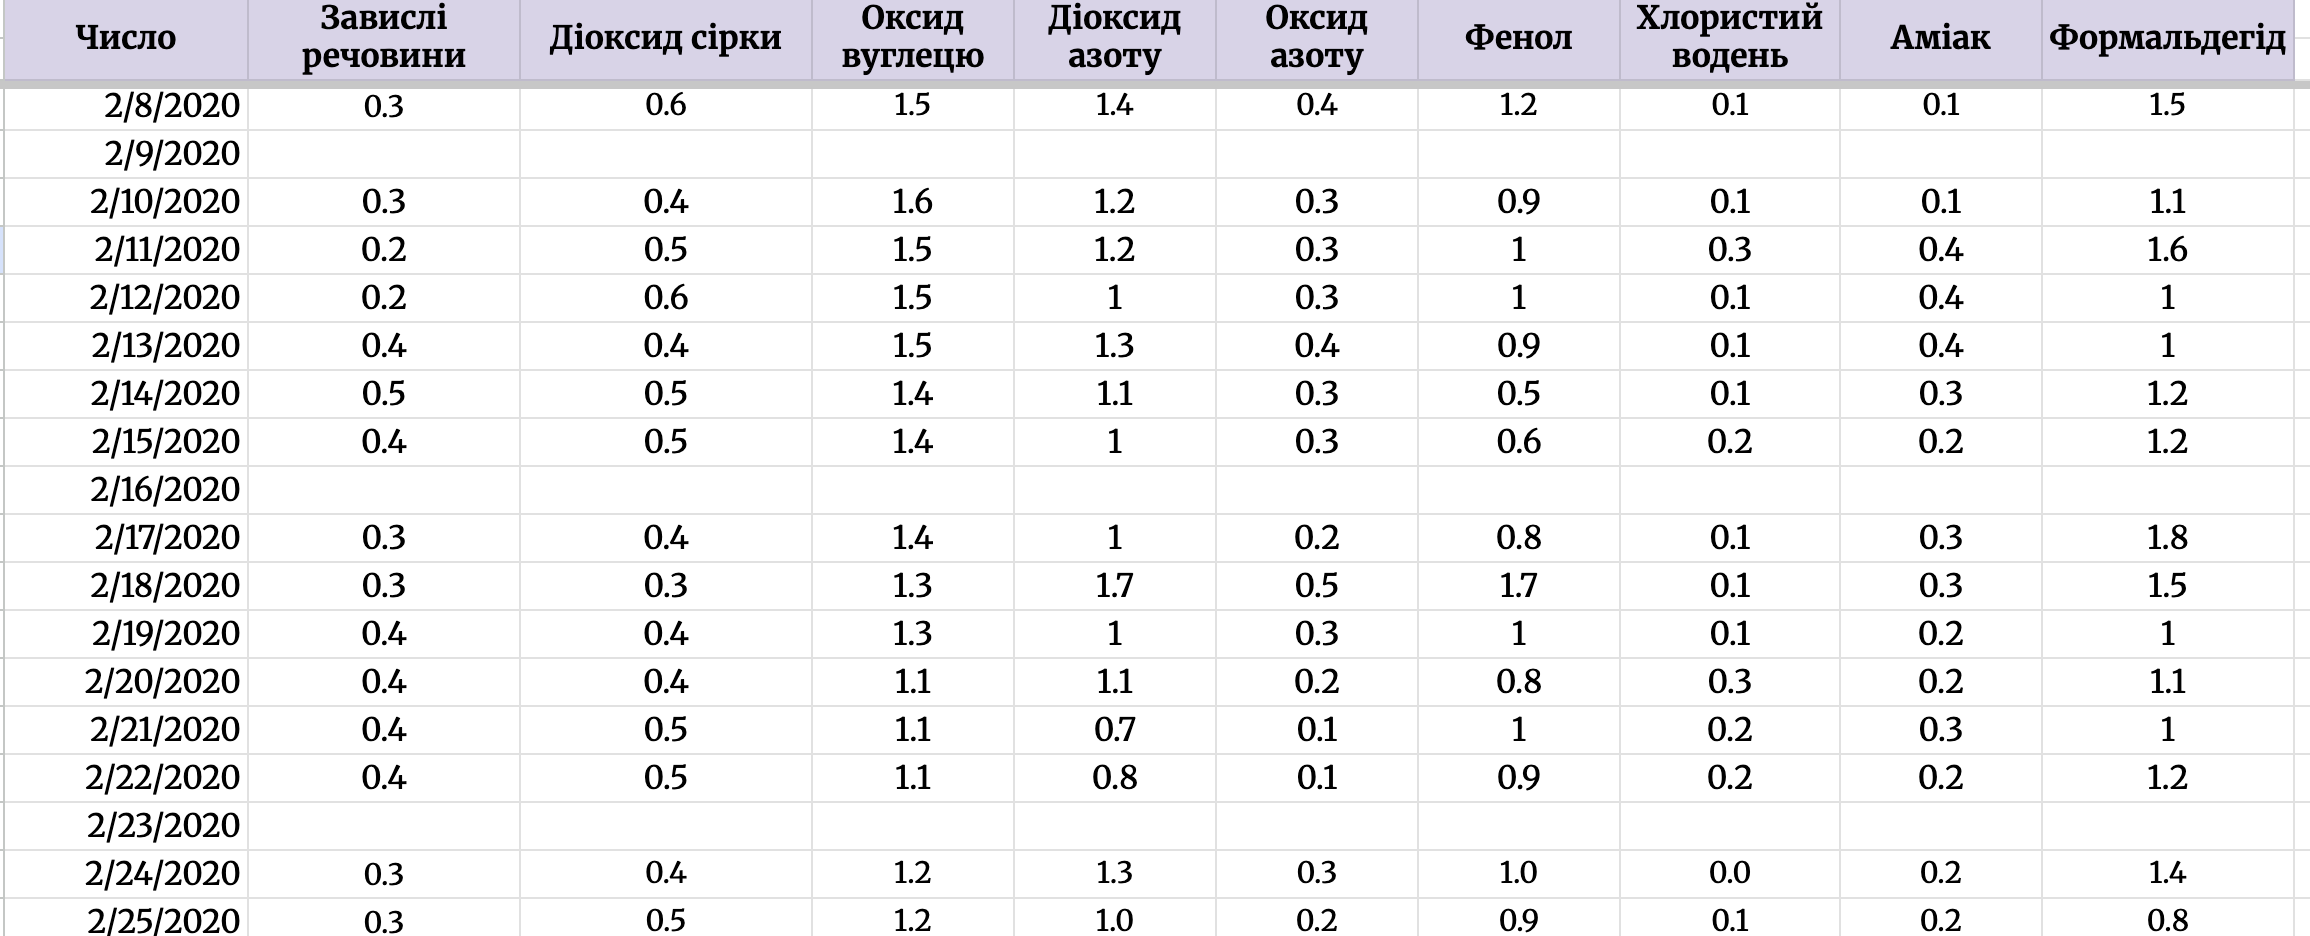
\includegraphics[width=0.8\textwidth]{images/dataset.png}
\caption{Приклад даних про забруднення повітря в Хмельницькому.}
\end{figure}

Міст сирої таблички даних прикріплений до роботи під 
назвою \textsf{khmelnytskyi.csv}. 

\subsection{Згладжування даних}

Для аналізу даних про забруднення повітря було застосовано метод згладжування
даних, який дозволяє заповнити пропуски в даних та зменшити вплив шуму.
Окрім того, деякі методи аналізу даних вимагають наявності гладких 
даних, тому згладжування є важливим етапом підготовки даних.

Для цього ми застосували наступний код на Python. Спочатку ми просто 
завантажуємо дані з CSV-файлу, конвертуємо колонки в числові значення та
парсимо дати. Потім, виділяємо колонки з забруднюючими речовинами.
\begin{minted}{python}
def load_and_preprocess_data(file_path: Path):
    """
    Loads the CSV data, converts columns to numeric, and parses dates.
    """
    
    try:
        df = pd.read_csv(file_path)
    except FileNotFoundError:
        print(f"Error: The file '{file_path}' was not found.")
        return None, None

    # Convert 'Date' column to datetime objects
    df['Date'] = pd.to_datetime(df['Date'], errors='coerce')
    # Remove rows where date conversion failed
    df = df.dropna(subset=['Date'])
    
    if df.empty:
        print("Error: No valid dates found after parsing. DataFrame is empty.")
        return None, None
    
    df = df.set_index('Date')

    # Identify pollutant columns
    pollutant_columns = df.columns.tolist()

    # Convert pollutant columns to numeric
    for col in pollutant_columns:
        df[col] = pd.to_numeric(df[col], errors='coerce')

    return df, pollutant_columns
\end{minted}

Також, додаємо метод для згладжування даних:
\begin{minted}{python}
def fill_all_gaps(df, pollutant_columns, method='linear'):
    """
    Fills all gaps in the specified columns using interpolation.
    """
    
    df_filled_all = df.copy()
    for col in pollutant_columns:
        df_filled_all[col] = df_filled_all[col].interpolate(method=method)
        
    return df_filled_all
\end{minted}

Тут використовується метод лінійної інтерполяції для заповнення пропусків в
даних (себто, якщо пропущене значення для часу $\tau \in (t_0,t_1)$ де відомі
послідовні значення $x(t_0)$ та $x(t_1)$, то ми заповнюємо його наступнм чином:
$x(\tau) = x(t_0) + \frac{(\tau - t_0)}{t_1 - t_0}(x(t_1)-x(t_0))$). Помітимо, 
що можна виокристовувати і більш складні методи згладжування, наприклад,
\textit{сплайн-інтерполяцію} або \textit{поліноміальну регресію}, але в нашому
випадку лінійна інтерполяція достатня для згладжування даних.

Результат згладжування даних збережено у
\texttt{khmelnytskyi\_filled\_all\_gaps.csv}. Приклад 
згладжених даних зображено на Рисунку~\ref{fig:smoothed_data}.

\begin{figure}[H]
\centering
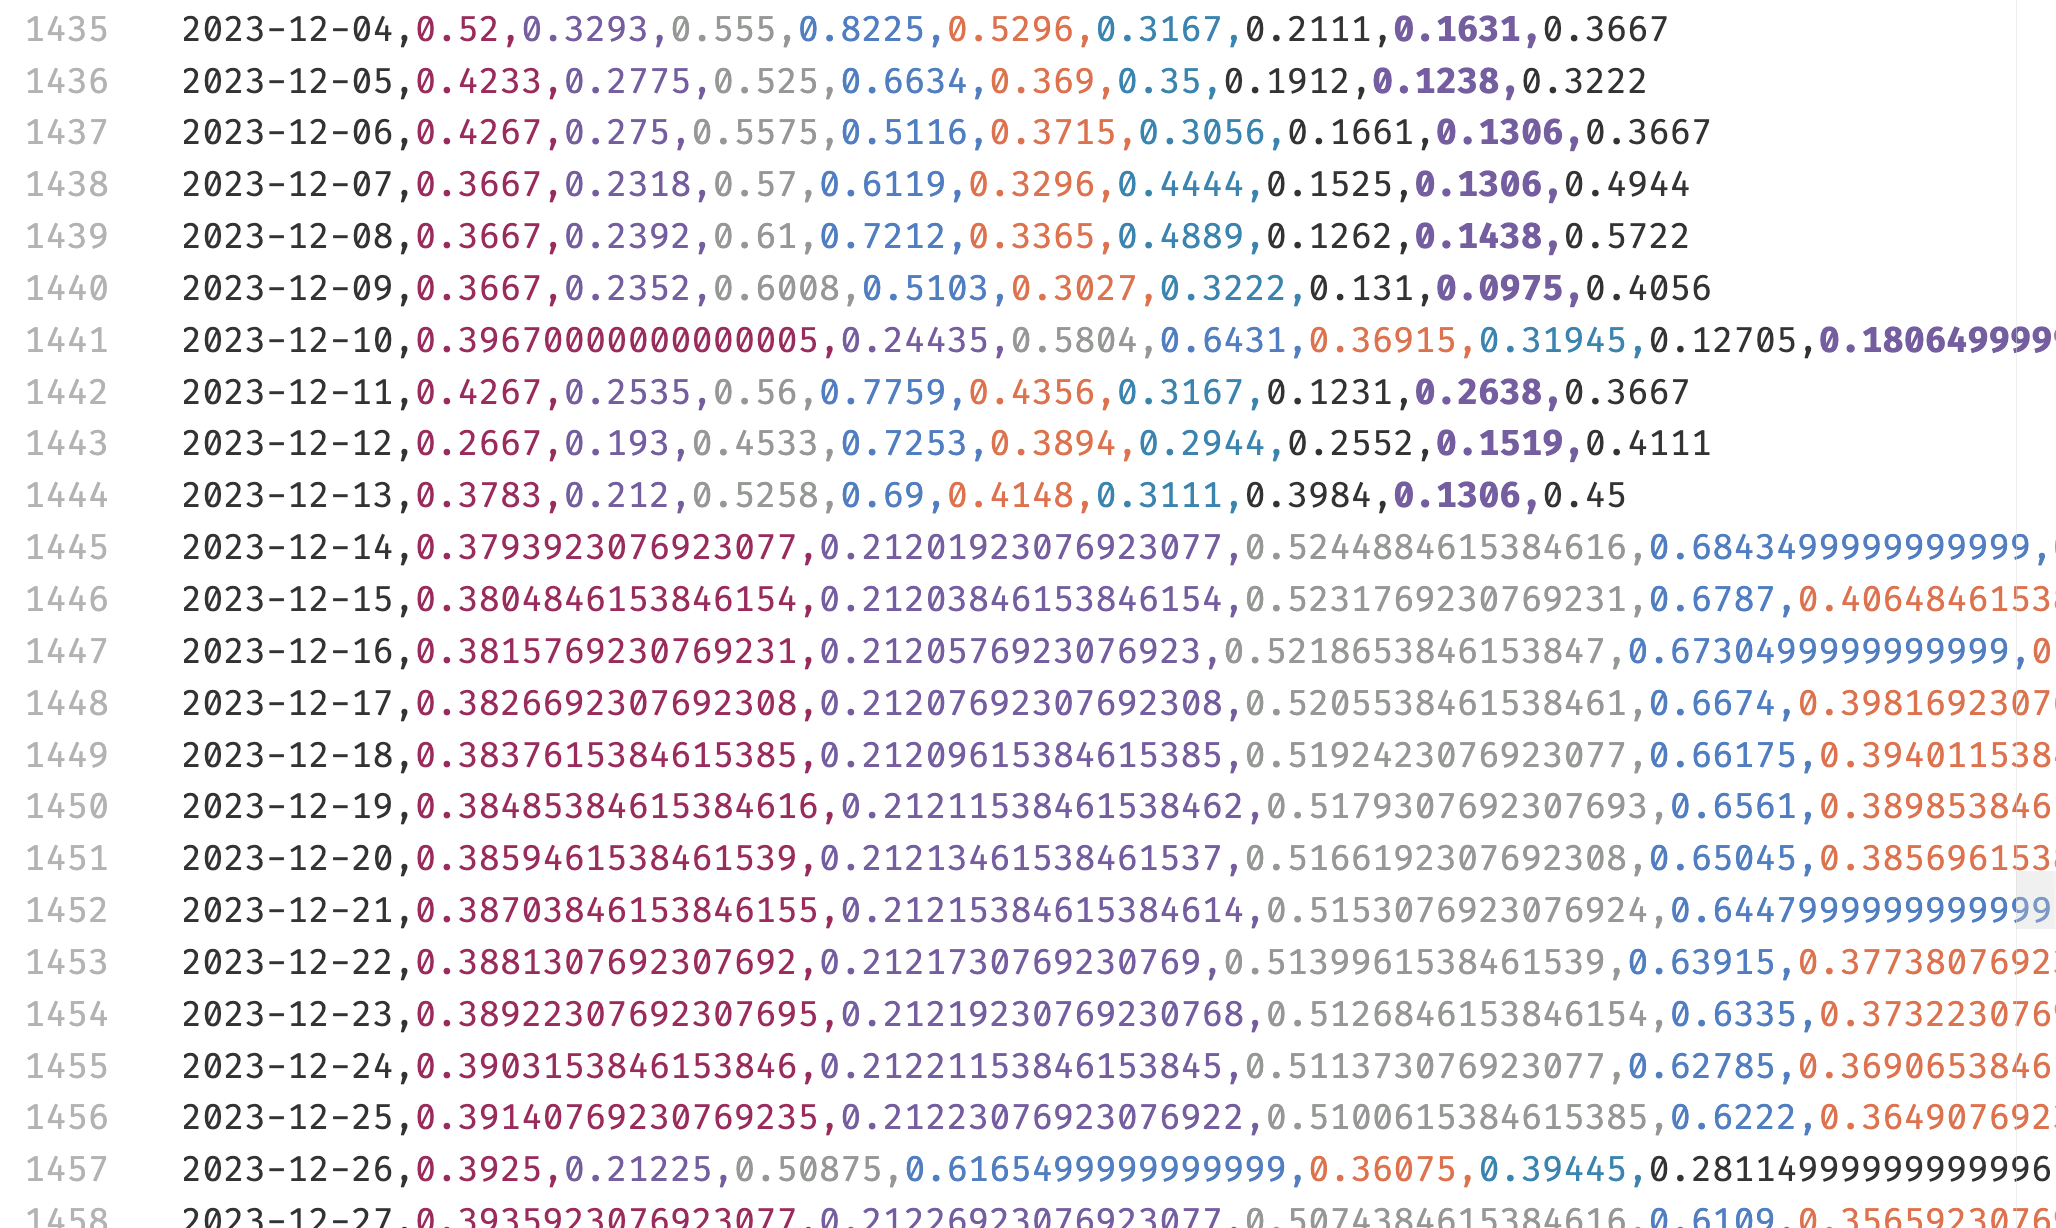
\includegraphics[width=0.8\textwidth]{images/dataset_interpolated.png}
\caption{Приклад згладжених даних.}
\label{fig:smoothed_data}
\end{figure}

\subsection{Дескриптивна статистика}

\subsubsection{Функції густини}
Тут ми можемо обрахувати деякі статистичні показники для кожної
забруднюючої речовини, наприклад, середнє значення, медіану, моду, дисперсію,
стандартне відхилення, коефіцієнт асиметрії та ексцесу. Також, ми робимо 
цей обрахунок по роках, щоб побачити, як змінюється рівень забруднення
протягом часу. Але для початку, давайте просто відобразимо функції 
густини для кожної забруднюючої речовини, щоб побачити їх розподіл.
Для цього виконаємо наступний код на Python:
\begin{minted}{python}
def plot_density_functions(df, pollutant_columns, output_dir="plots/density_functions"):
    """
    Generates and saves probability density function (PDF/KDE) plots
    for each pollutant in separate files.
    """
    
    if df.empty:
        print("DataFrame is empty. No density plots will be generated.")
        return

    # Ensure the output directory exists
    output_path = Path(output_dir)
    output_path.mkdir(parents=True, exist_ok=True)
    print(f"Ensured directory exists: {output_path}")

    # Iterate through each pollutant column
    for col in pollutant_columns:
        plt.figure(figsize=(10, 6))
        data_series = df[col].dropna()

        # Check if there is data left to plot
        if data_series.empty:
            print(f"No data for pollutant '{col}'. Skipping density plot.")
            plt.close()
            continue

        # Create the Kernel Density Estimate plot using seaborn
        sns.kdeplot(data_series, fill=True, bw_adjust=0.75)

        # Customize the plot
        plt.title(f'Probability Density Function for {col}', fontsize=14)
        plt.xlabel(f'{col} Value (Concentration)', fontsize=10)
        plt.ylabel('Density', fontsize=10)
        plt.grid(True, linestyle='--', alpha=0.6)
        plt.tight_layout()

        # Prepare filename
        safe_col_name = col.replace(' ', '_').replace('/', '_').lower()
        plot_filename = f"density_{safe_col_name}.pdf"
        full_plot_path = output_path / plot_filename

        # Save the plot
        try:
            plt.savefig(full_plot_path, dpi=300, format='pdf', bbox_inches='tight')
            print(f"Saved density plot to: {full_plot_path}")
        except Exception as e:
            print(f"Error saving plot for {col}: {e}")

        plt.close()  
\end{minted}

Отримаємо наступні графіки функцій густини для кожної забруднюючої речовини:
див. Рисунок~\ref{fig:pdfs}. Як бачимо, деякі забруднюючі речовини мають
розподіл, близький до нормального, в той час як інші мають більш складний
розподіл з декількома піками. Це може свідчити про наявність різних джерел
забруднення або про сезонні коливання в рівні забруднення повітря (визначення
цих джерел та сезонних коливань виходить за межі цієї роботи і взагалі роботи
математика/статистика).

\begin{figure}
    \begin{tabular}{ccc}
      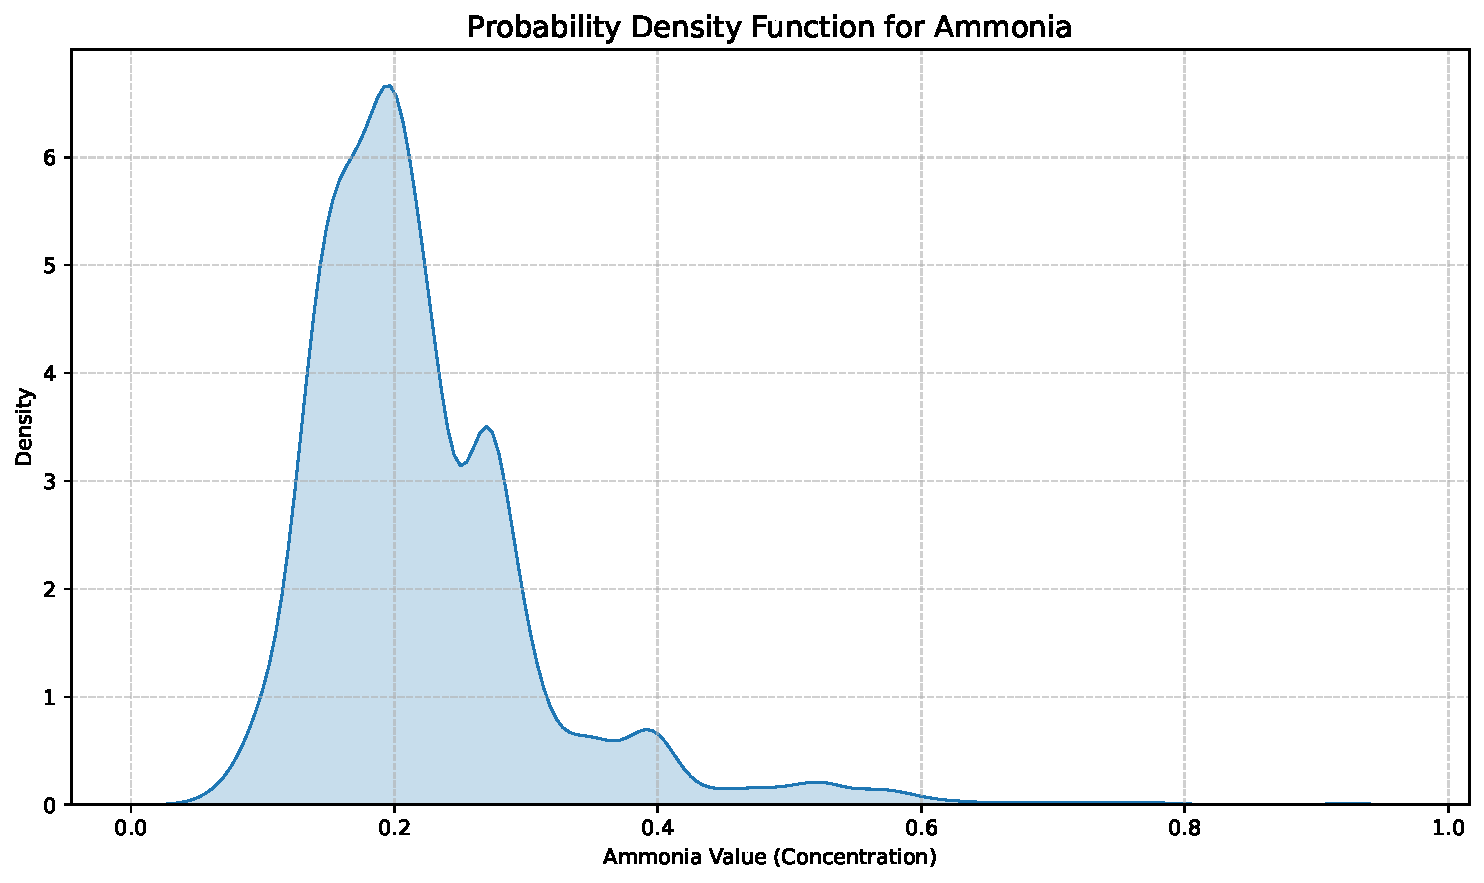
\includegraphics[width=0.33\textwidth]{../plots/khmelnytskyi_stats_plots/density_functions/density_ammonia.pdf} & 
      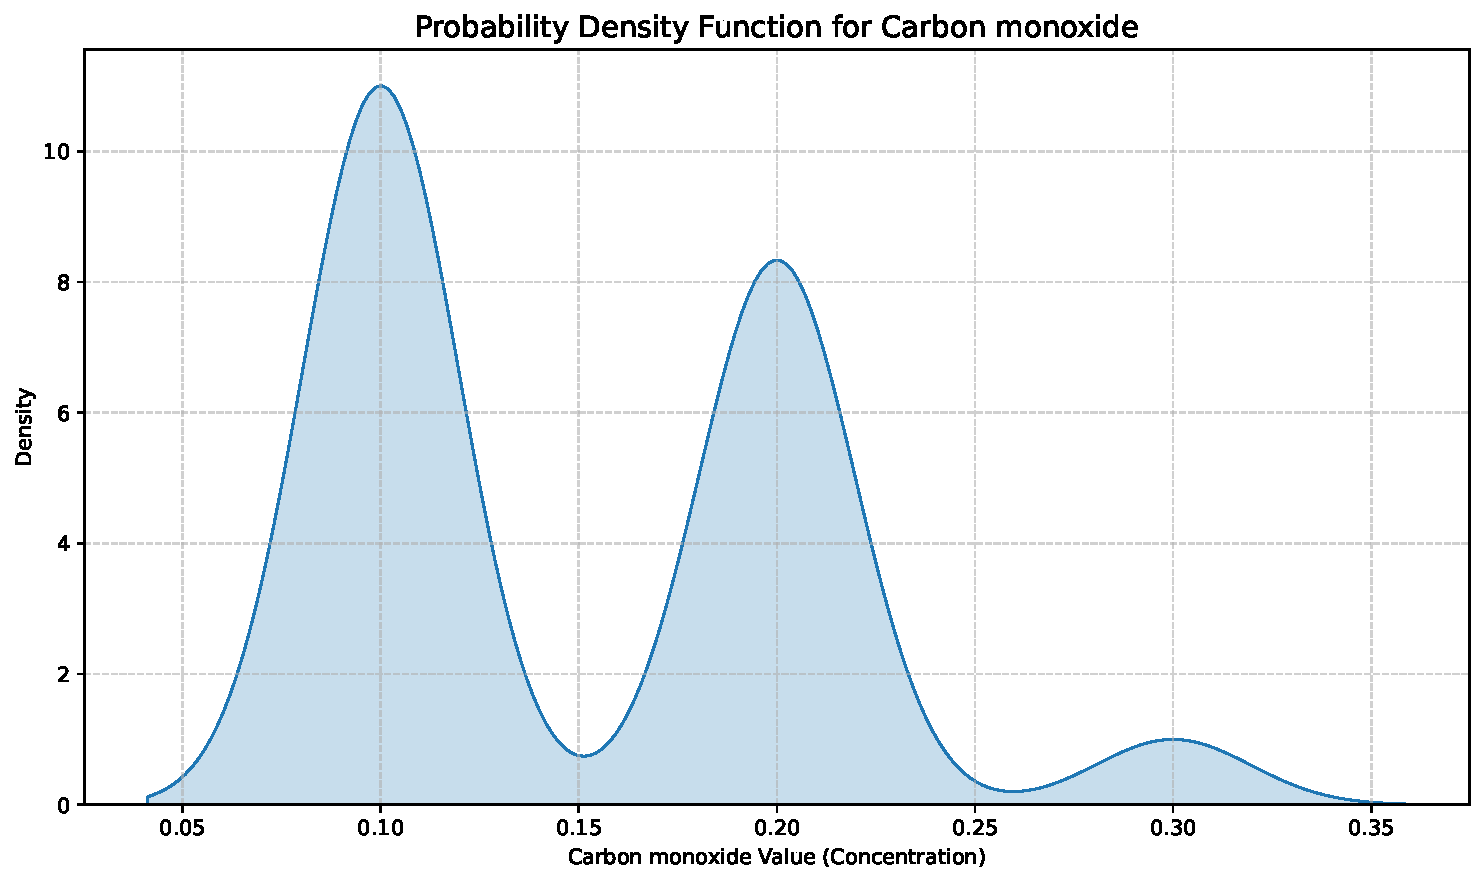
\includegraphics[width=0.33\textwidth]{../plots/khmelnytskyi_stats_plots/density_functions/density_carbon_monoxide.pdf} &
      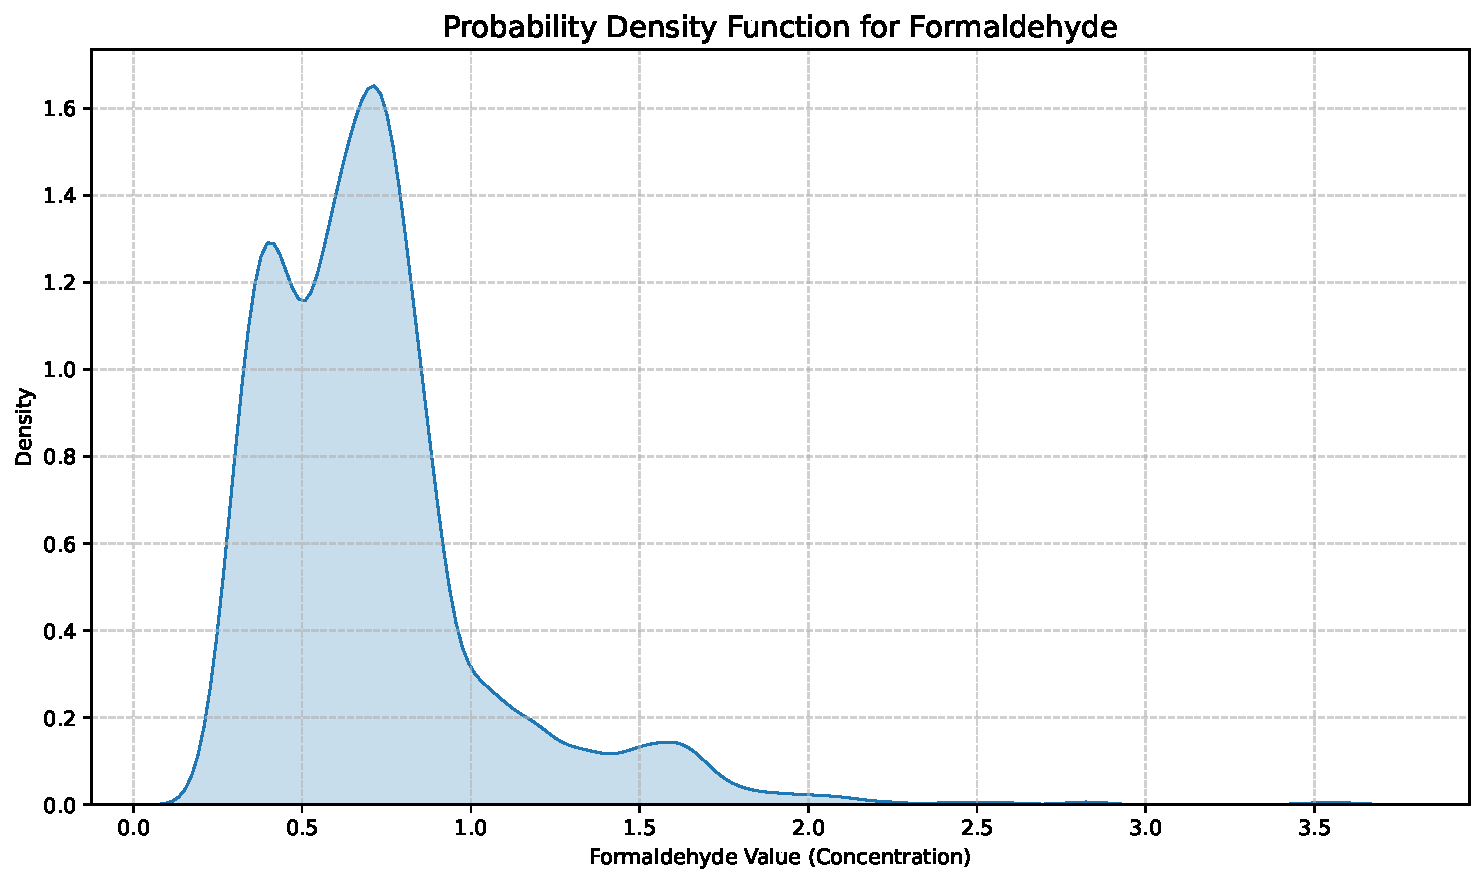
\includegraphics[width=0.33\textwidth]{../plots/khmelnytskyi_stats_plots/density_functions/density_formaldehyde.pdf} \\
      Ammonia & Carbon Monoxide & Formaldehyde \\
      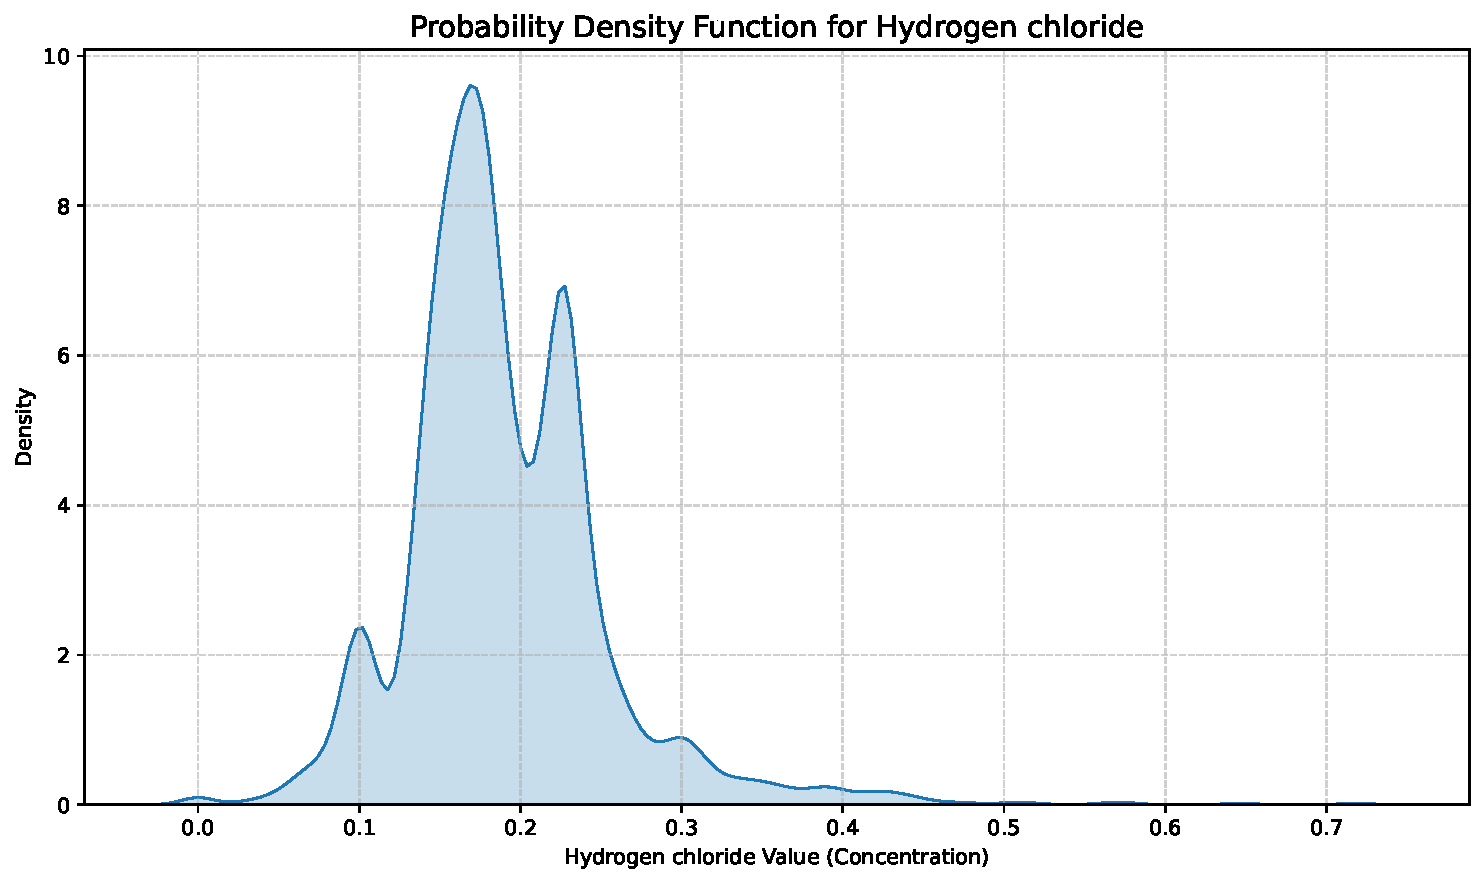
\includegraphics[width=0.33\textwidth]{../plots/khmelnytskyi_stats_plots/density_functions/density_hydrogen_chloride.pdf} &
      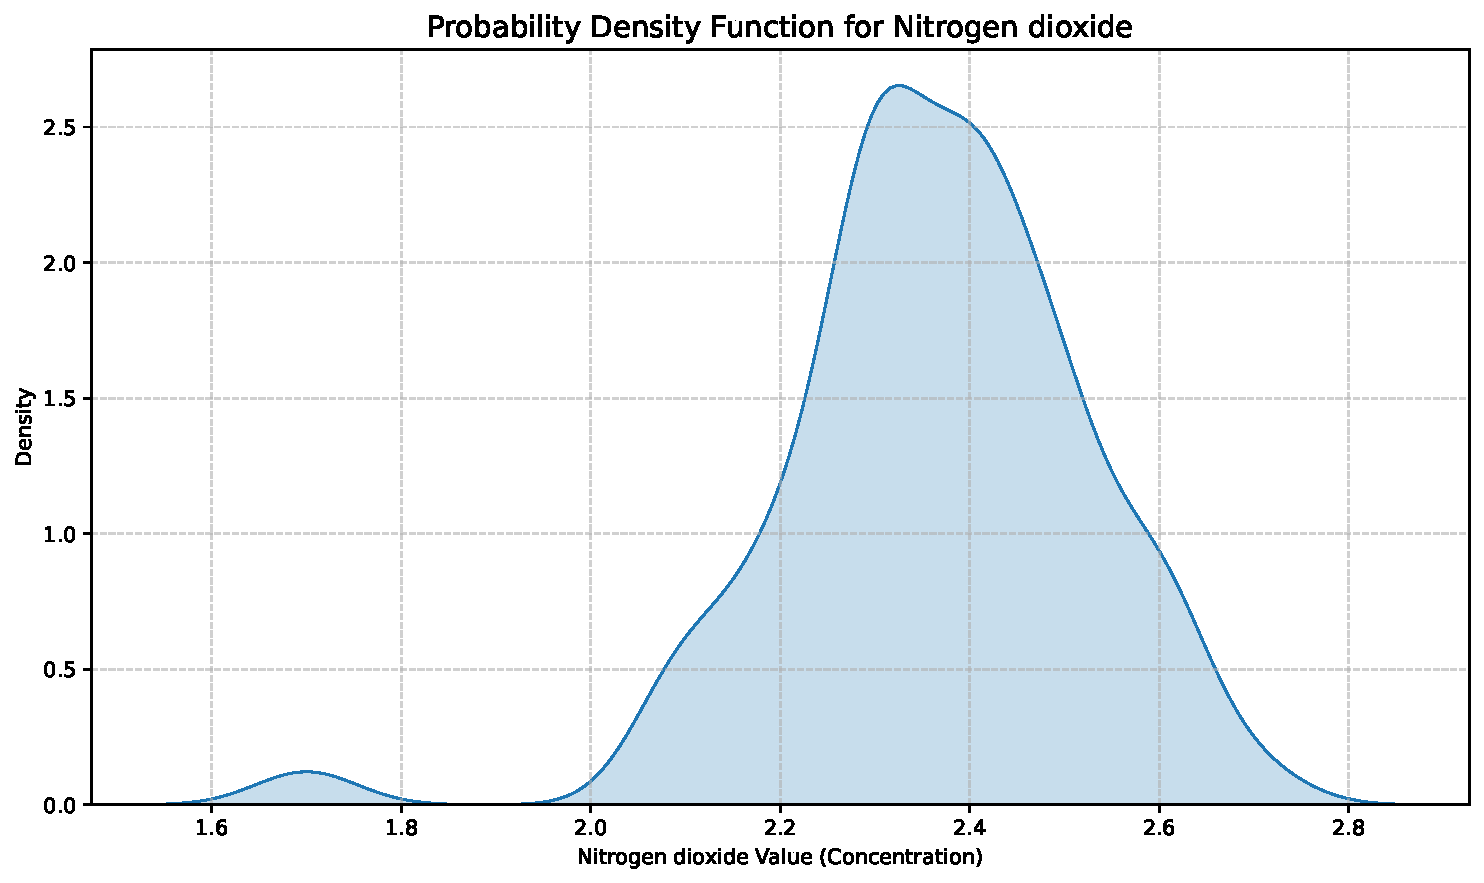
\includegraphics[width=0.33\textwidth]{../plots/khmelnytskyi_stats_plots/density_functions/density_nitrogen_dioxide.pdf} &
      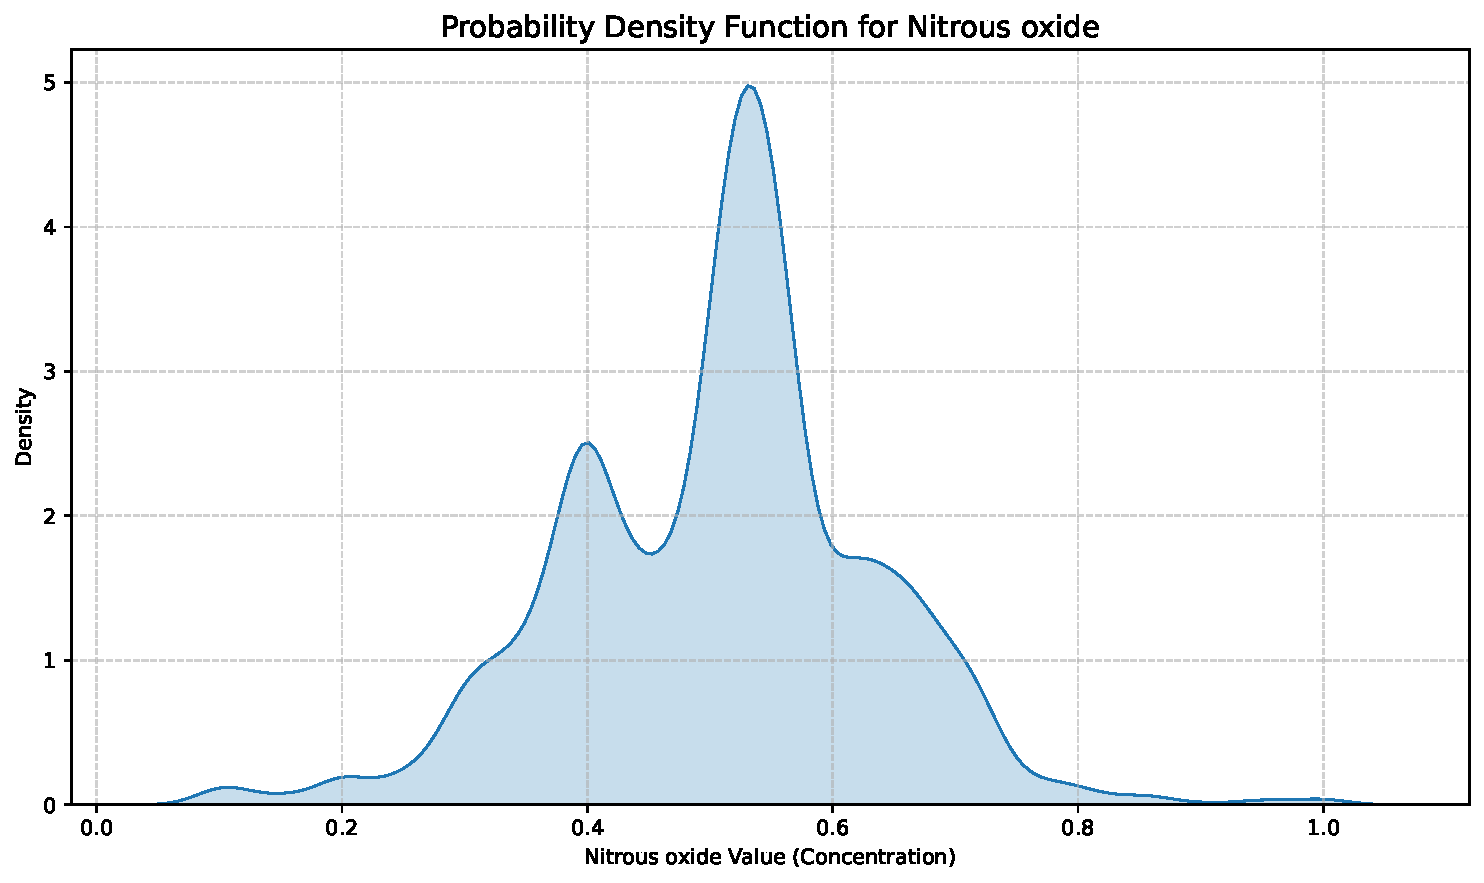
\includegraphics[width=0.33\textwidth]{../plots/khmelnytskyi_stats_plots/density_functions/density_nitrous_oxide.pdf} \\
        Hydrogen Chloride & Nitrogen Dioxide & Nitrous Oxide \\
      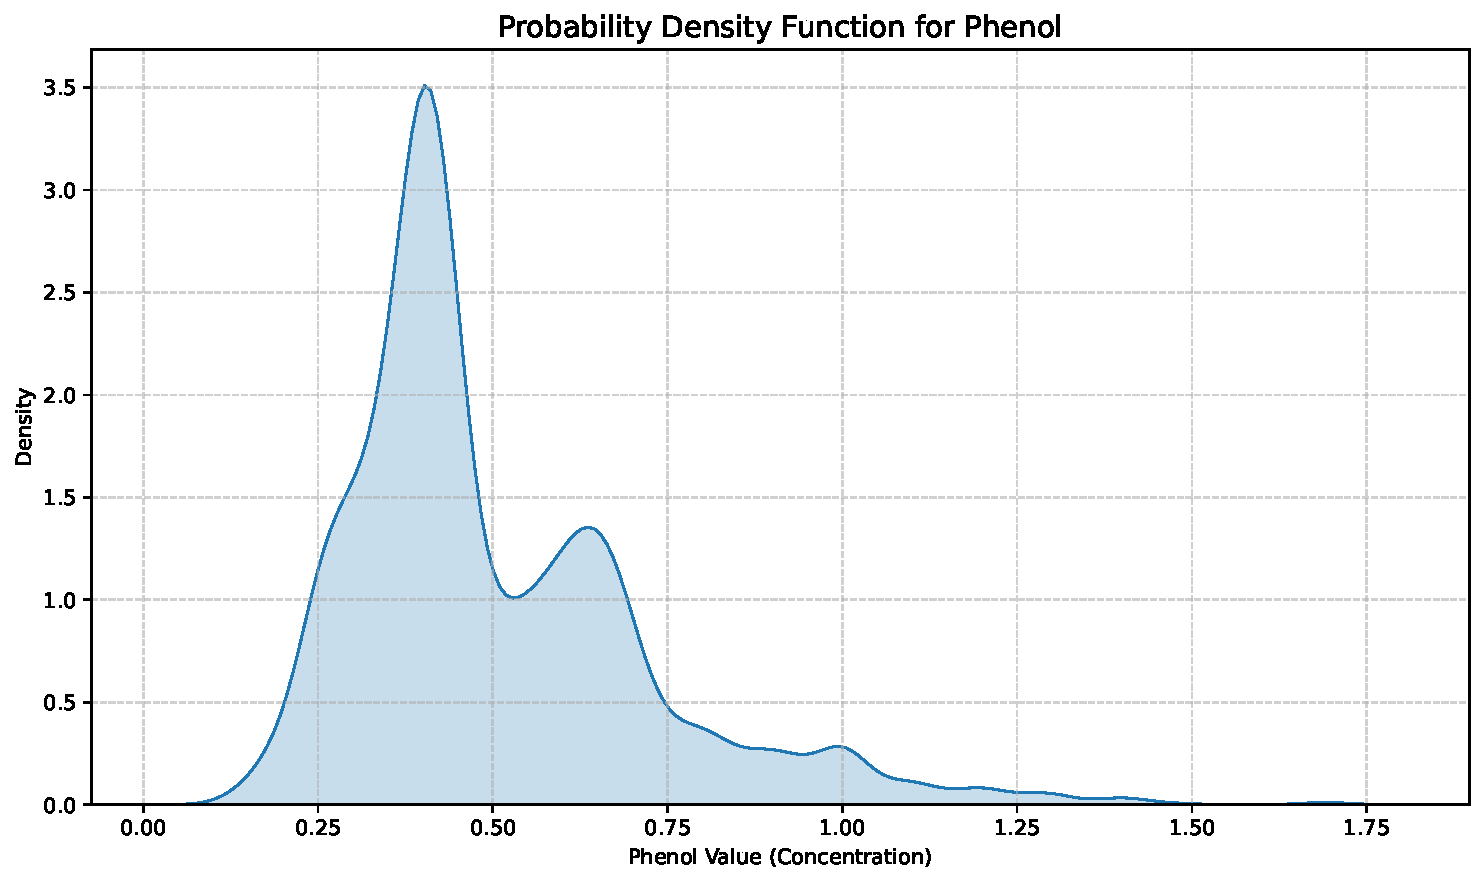
\includegraphics[width=0.33\textwidth]{../plots/khmelnytskyi_stats_plots/density_functions/density_phenol.pdf} &
      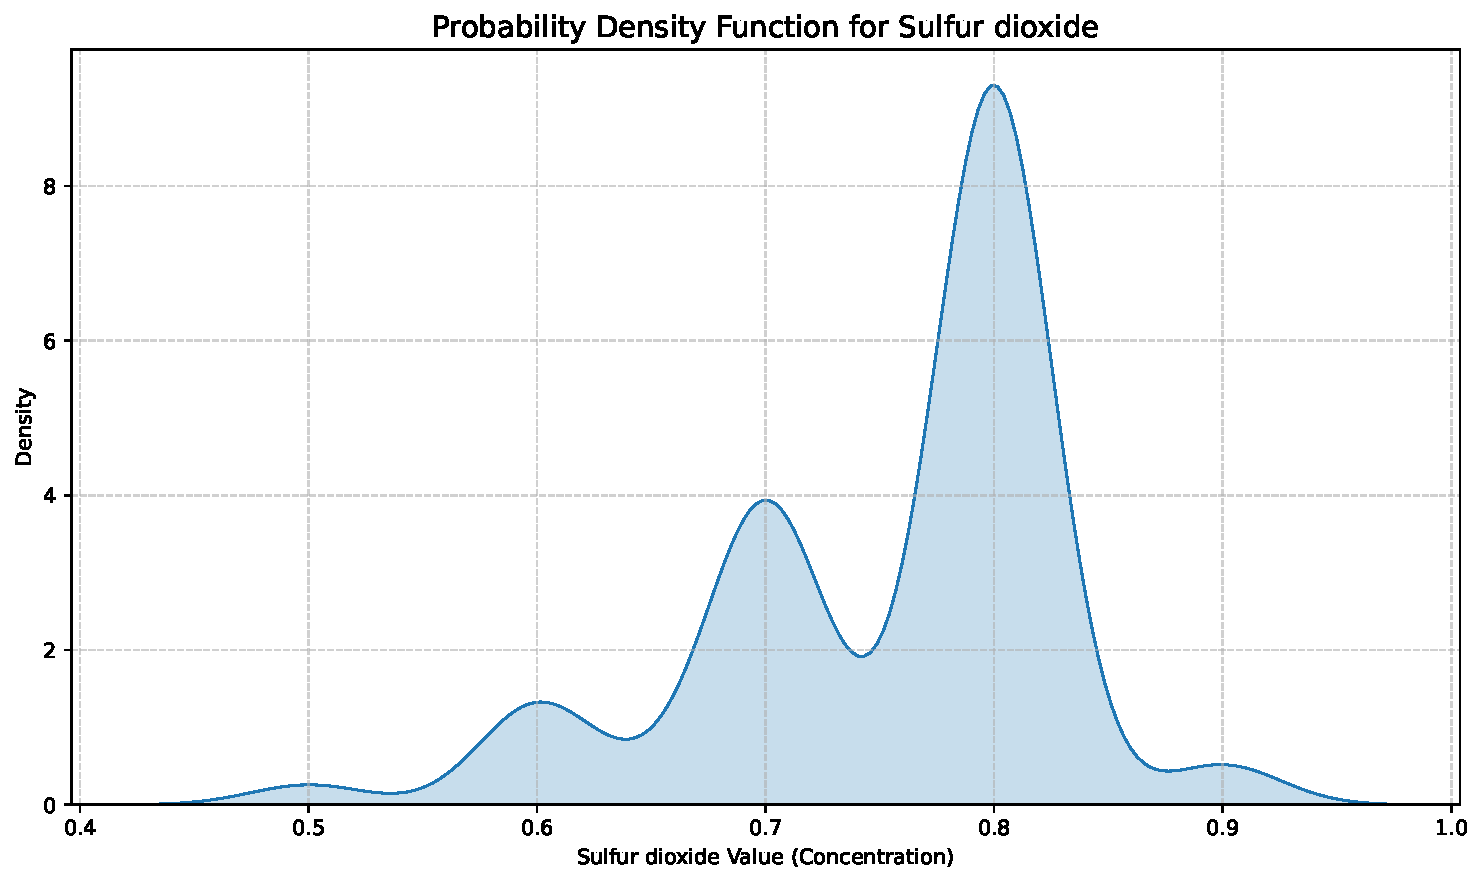
\includegraphics[width=0.33\textwidth]{../plots/khmelnytskyi_stats_plots/density_functions/density_sulfur_dioxide.pdf} &
      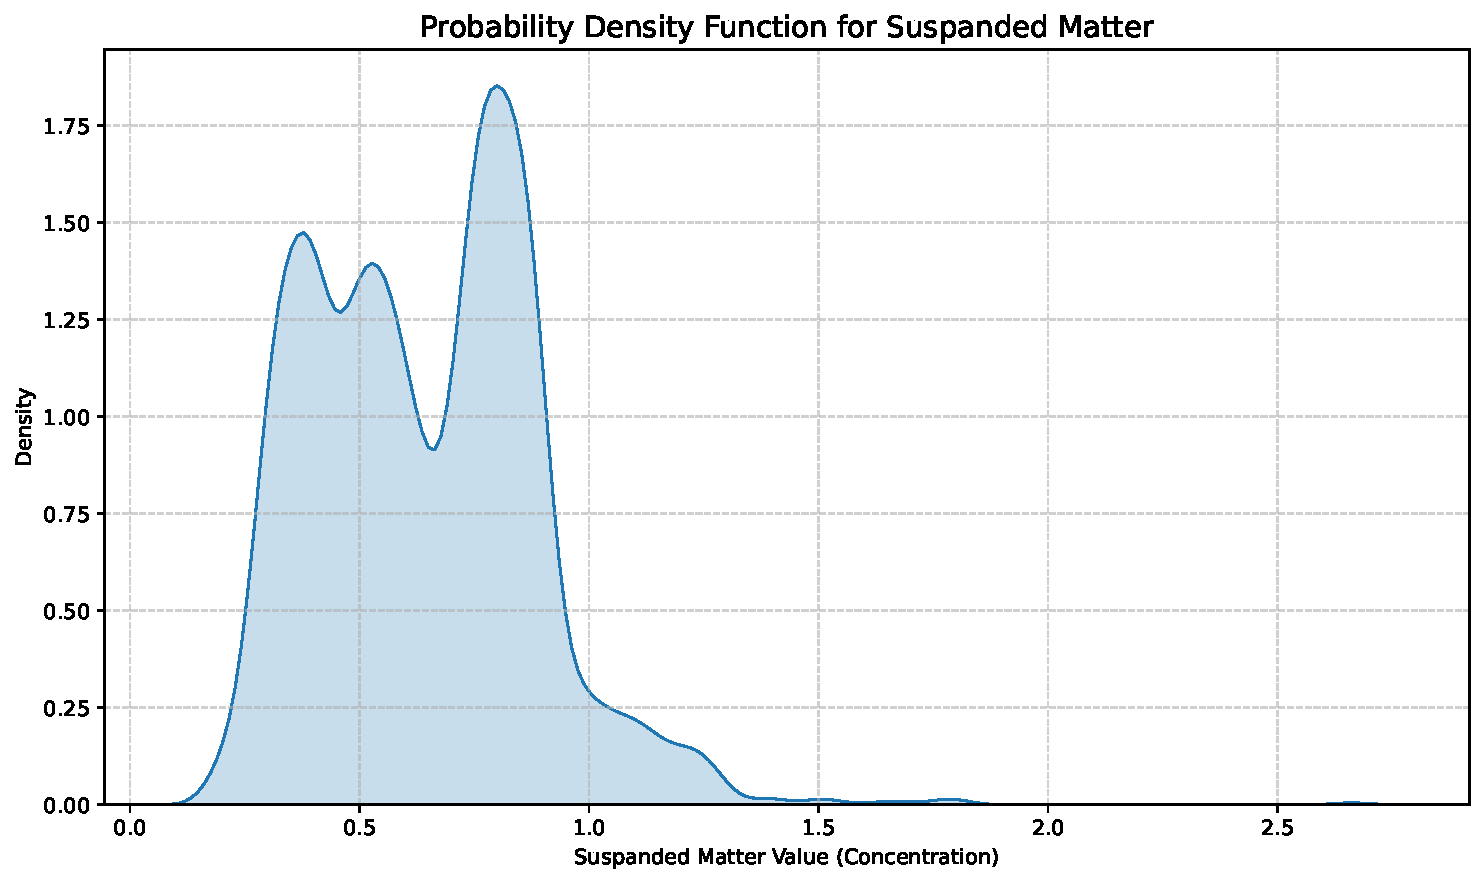
\includegraphics[width=0.33\textwidth]{../plots/khmelnytskyi_stats_plots/density_functions/density_suspanded_matter.pdf} \\
        Phenol & Sulfur Dioxide & Suspended Matter \\
    \end{tabular}
    \caption{Графіки функцій густини для кожної забруднюючої речовини}
    \label{fig:pdfs}
\end{figure}

\subsubsection{Статистичні показники}

Тепер ми можемо обрахувати деякі статистичні показники для кожної 
забруднюючої речовини. Для цього ми можемо використати наступний код на Python:
\begin{minted}{python}
def calculate_descriptive_stats(df, pollutant_columns):
    """
    Calculates descriptive statistics for each pollutant, grouped by year and overall.
    """
    
    all_stats = []

    if df.empty or df.index.empty:
        print("Warning: DataFrame is empty or has no valid DatetimeIndex. Cannot calculate yearly stats.")
        return pd.DataFrame()

    if not isinstance(df.index, pd.DatetimeIndex):
        print("Warning: Index is not a DatetimeIndex. Cannot extract year.")
        
        try:
            df.index = pd.to_datetime(df.index)
        except Exception as e:
            print(f"Error converting index to DatetimeIndex: {e}")
            return pd.DataFrame()

    df_with_year = df.copy()
    df_with_year['Year'] = df_with_year.index.year

    if df_with_year['Year'].isnull().all():
        print("Warning: Could not extract valid years from the DataFrame index.")
        years = []
    else:
        years = sorted(df_with_year['Year'].dropna().unique().astype(int))

    for col in pollutant_columns:
        # Overall statistics
        data_series = df_with_year[col].dropna()
        if not data_series.empty:
            mode_result = stats.mode(data_series, keepdims=True)
            mode_val = mode_result.mode[0] if mode_result.mode.size > 0 else np.nan

            stats_dict = {
                'Pollutant': col,
                'Year': 'Overall',
                'Mean': data_series.mean(),
                'Median': data_series.median(),
                'Mode': mode_val,
                'Min': data_series.min(),
                'Max': data_series.max(),
                'Kurtosis': data_series.kurtosis(),
                'Skewness': data_series.skew(),
                'Std Dev': data_series.std()
            }
            all_stats.append(stats_dict)

        # Per-year statistics
        for year in years:
            year_data = df_with_year[df_with_year['Year'] == year][col].dropna()
            if not year_data.empty:
                mode_result_year = stats.mode(year_data, keepdims=True)
                mode_val_year = mode_result_year.mode[0] if mode_result_year.mode.size > 0 else np.nan

                stats_dict_year = {
                    'Pollutant': col,
                    'Year': str(year),
                    'Mean': year_data.mean(),
                    'Median': year_data.median(),
                    'Mode': mode_val_year,
                    'Min': year_data.min(),
                    'Max': year_data.max(),
                    'Kurtosis': year_data.kurtosis(),
                    'Skewness': year_data.skew(),
                    'Std Dev': year_data.std()
                }
                all_stats.append(stats_dict_year)

    stats_df = pd.DataFrame(all_stats)
    if not stats_df.empty:
        stats_df['Year'] = stats_df['Year'].astype(str)
        stats_df = stats_df.set_index(['Pollutant', 'Year'])
    
    return stats_df
\end{minted}

Як бачимо, ми обраховуємо наступні показники:
\begin{itemize}
    \item \textbf{Середнє значення} (Mean) --- середнє арифметичне значення. За 
    деталями див. Розділ~\ref{sec:mean}.
    \item \textbf{Медіана та модна} (Median \& Mode) --- за деталями див.
    Розділ~\ref{sec:median_mode}.
    \item \textbf{Мінімальне та максимальне значення} (Min \& Max) --- найменше
    та найбільше значення в даних відповідно.
    \item \textbf{Коефіцієнт асиметрії та ексцесу} (Skewness \& Kurtosis) ---
    за деталями див. Розділ~\ref{sec:kurtosis_skewness}.
    \item \textbf{Стандартне відхилення} (Std Dev) --- міра розсіювання даних
    навколо середнього значення. За деталями див. Розділ~\ref{sec:dispersion}.
\end{itemize}

Ми зберегли усі показники в CSV-файл
\texttt{khmelnytskyi\_descriptive\_stats.csv}, який містить статистику по кожній
забруднюючій речовині та по роках. Приклад отриманої таблиці зображено на
Рисунку~\ref{fig:descriptive_stats}.

\begin{figure}[H]
\centering
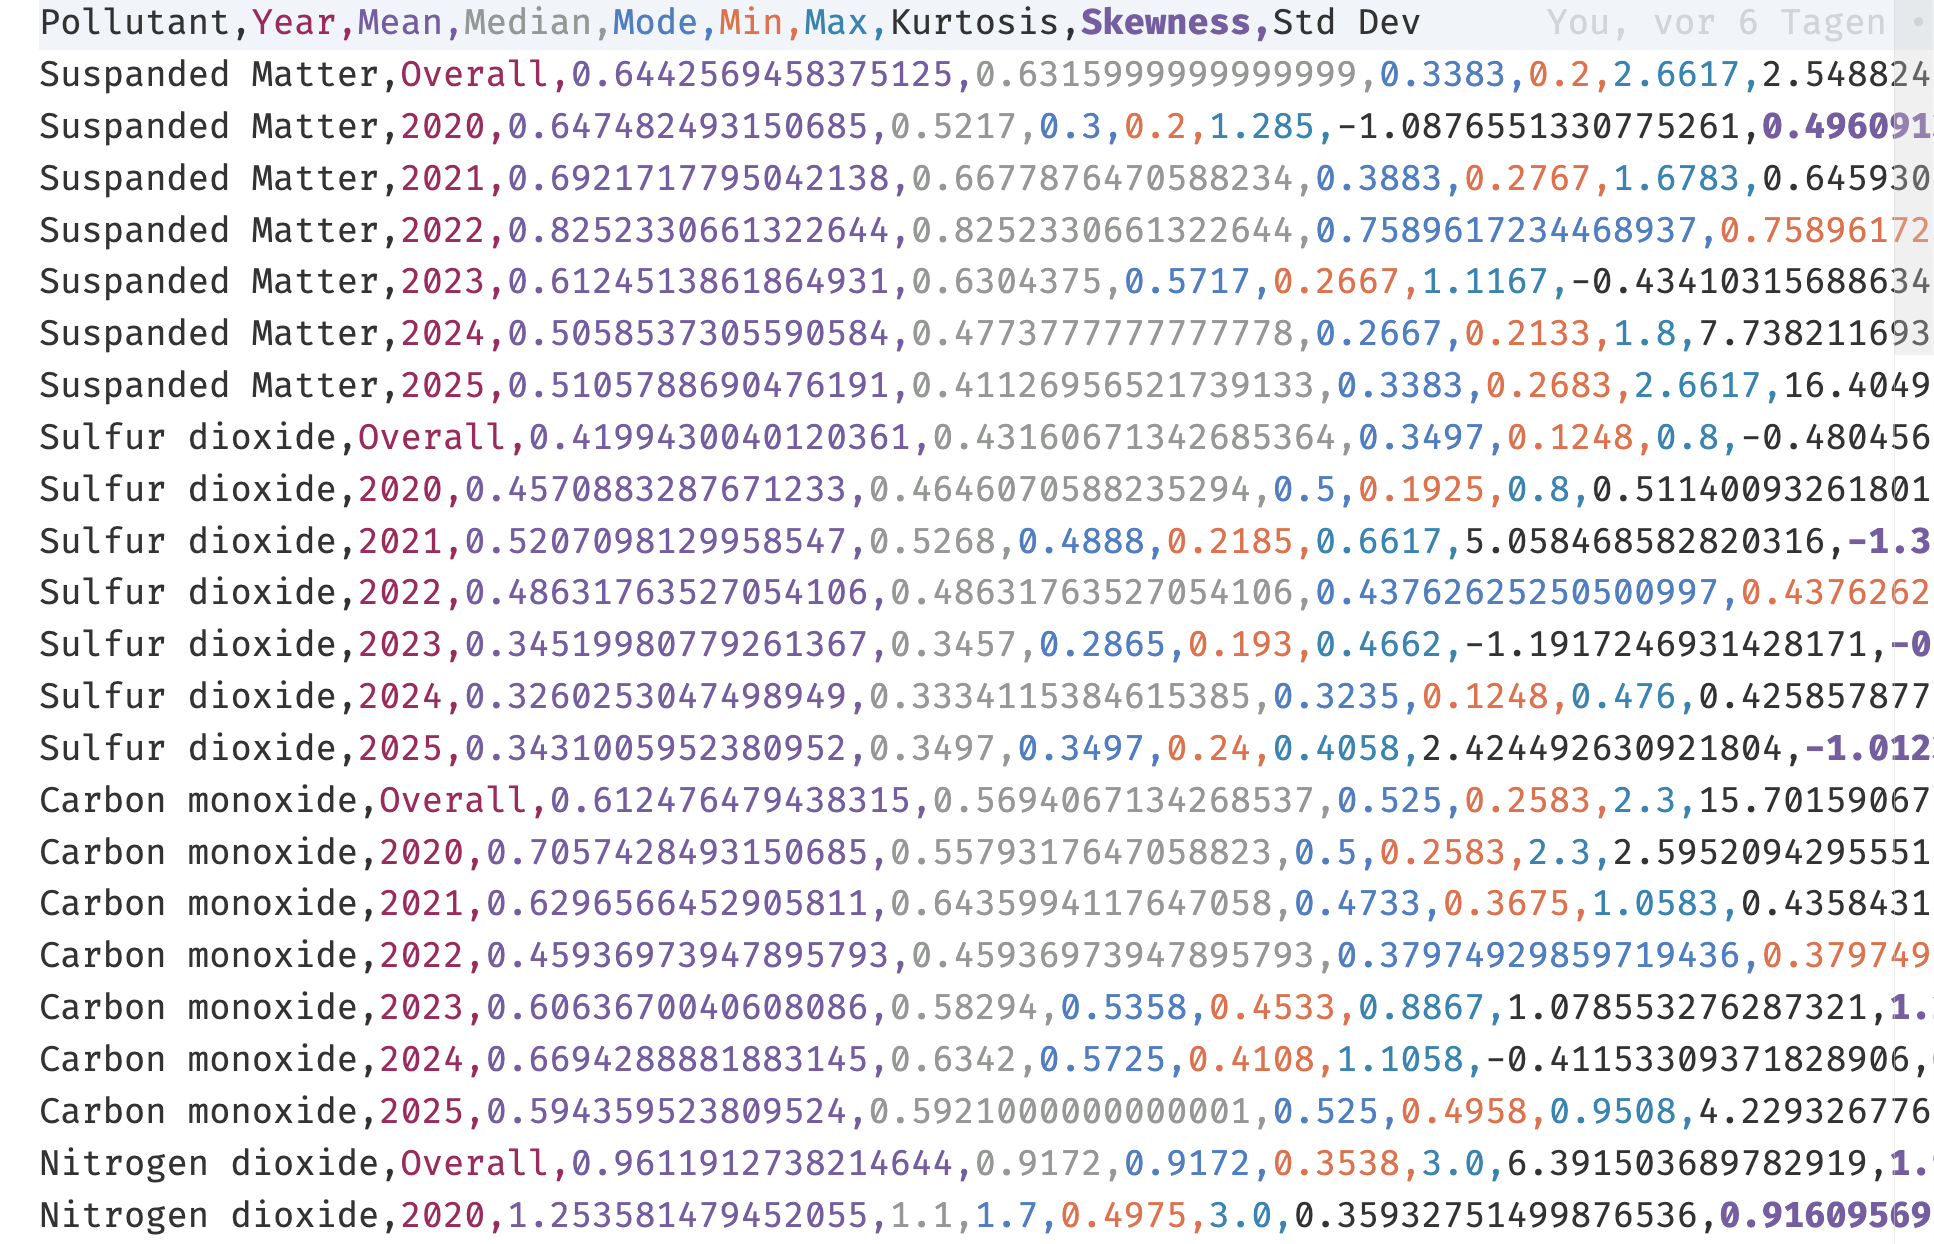
\includegraphics[width=0.8\textwidth]{images/descriptive_stats.png}
\caption{Приклад статистичних показників для забруднюючих речовин в Хмельницькому.}
\label{fig:descriptive_stats}
\end{figure}

Візуалізуємо ці показники. Найбільш репрезентативним з них є середнє 
значення по роках, яке показує, як змінюється середній рівень забруднення
протягом часу. Для цього ми можемо використати наступний код на Python:
\begin{minted}{python}
def plot_yearly_means_grouped(stats_df, output_dir="plots"):
    """
    Generates and saves a single grouped bar plot showing mean pollutant levels
    for each year. 
    """
    
    if stats_df.empty:
        print("Statistics DataFrame is empty. No plot will be generated.")
        return

    output_path = Path(output_dir)
    if not output_path.exists():
        os.makedirs(output_path)
        print(f"Created directory: {output_path}")

    try:
        # 1. Prepare data
        mean_stats = stats_df['Mean'].reset_index()
        mean_stats_yearly = mean_stats[mean_stats['Year'] != 'Overall'].copy()

        if mean_stats_yearly.empty:
            print("No yearly data found to plot.")
            return

        # 2. Ensure 'Year' is numeric for sorting, then convert back to string
        mean_stats_yearly['Year'] = pd.to_numeric(mean_stats_yearly['Year'])
        mean_stats_yearly = mean_stats_yearly.sort_values('Year')
        mean_stats_yearly['Year'] = mean_stats_yearly['Year'].astype(str)

        # 3. Pivot data for grouped bar chart (Years as index, Pollutants as columns)
        plot_data = mean_stats_yearly.pivot(index='Year', columns='Pollutant', values='Mean')

        if plot_data.empty:
            print("Could not pivot data for plotting.")
            return

        # 4. Create the plot
        num_years = len(plot_data.index)
        fig_width = max(14, num_years * 1.5)
        _ = plot_data.plot(kind='bar', figsize=(fig_width, 8), width=0.8)

        # 5. Setting plot design
        plt.title('Mean Pollutant Levels by Year in Khmelnytskyi', fontsize=16)
        plt.xlabel('Year', fontsize=12)
        plt.ylabel('Mean Value (Concentration / Index)', fontsize=12)
        plt.xticks(rotation=45, ha='right')
        plt.legend(title='Pollutants', bbox_to_anchor=(1.02, 1), loc='upper left')
        plt.grid(axis='y', linestyle='--', alpha=0.7)
        plt.tight_layout(rect=[0, 0, 0.88, 1])

        # 6. Define the output filename and path
        plot_filename = "yearly_mean_grouped_by_pollutant.pdf"
        full_plot_path = output_path / plot_filename

        # 7. Save the plot as PDF
        plt.savefig(full_plot_path, dpi=300, format='pdf', bbox_inches='tight')
        plt.close()
        print(f"Saved grouped bar plot to: {full_plot_path}")
        
    except KeyError as e:
        print(f"Error: Could not find expected column for plotting: {e}")
    except Exception as e:
        print(f"An error occurred while generating the grouped bar plot: {e}")
\end{minted}

Результат зображено на Рисунку~\ref{fig:yearly_means}.

\begin{figure}[H]
\centering
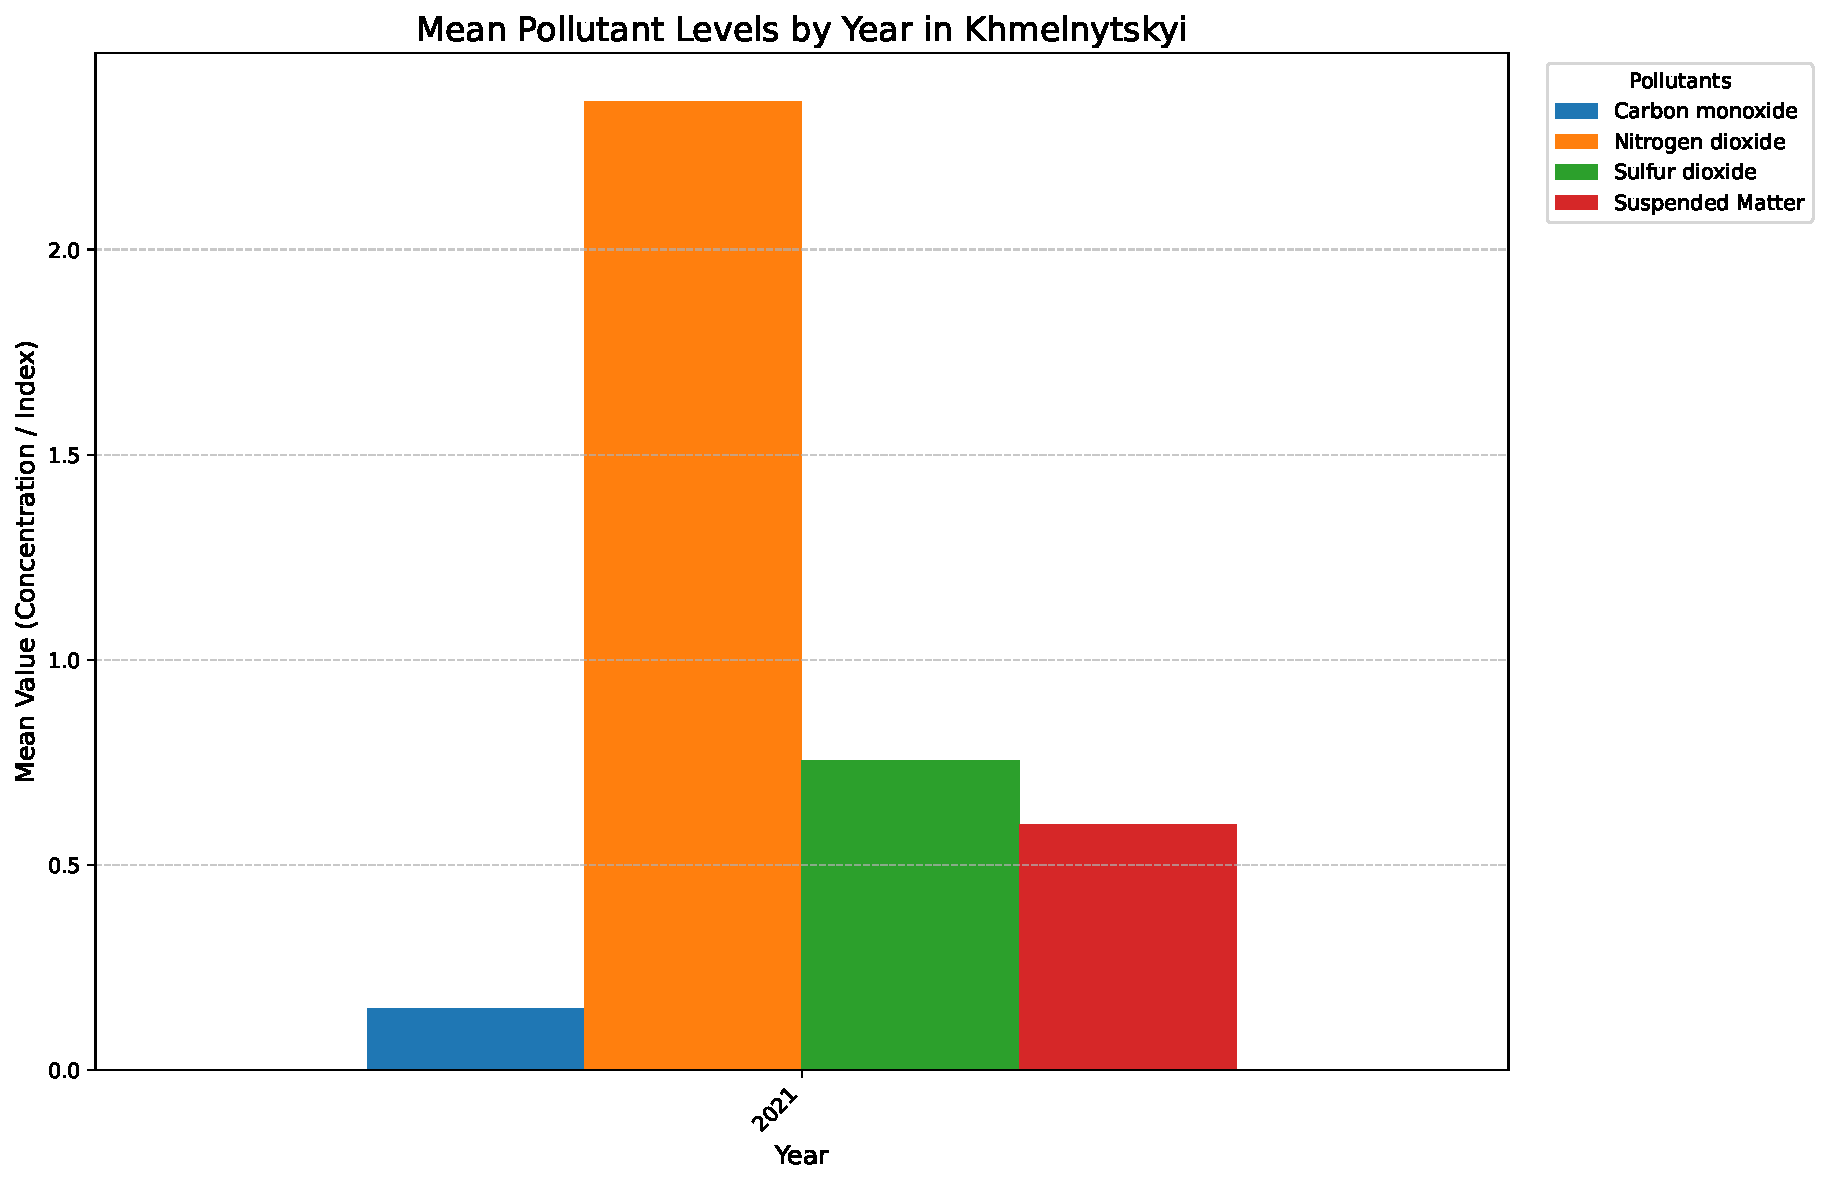
\includegraphics[width=\textwidth]{../plots/khmelnytskyi_stats_plots/yearly_mean_grouped_by_pollutant.pdf}
\caption{Групований стовпчиковий графік середніх значень забруднюючих речовин
по роках. Як бачимо, рівень забруднення повітря в Хмельницькому має тенденцію до
зниження протягом 2020---2023, зокрема, рівень формальдегіду та фенолу. Після 
цього, багато показників коливаються в межах одного рівня (наприклад, той самий 
фенол або, скажімо, nitrogen dioxide).}

\label{fig:yearly_means}
\end{figure}

Також ми вирішили порівняти середні значення забруднюючих речовин
між собою, щоб побачити, які з них є найбільш концентрованими в 
регіоні Хмельницького. Для цього ми можемо використати наступний код на Python:
\begin{minted}{python}
def plot_overall_means_pdf(stats_df, output_dir="plots"):
    """
    Generates and saves a single plot comparing the 'Overall' mean
    values across all pollutants. Saves as PDF with 300 dpi.
    """
    
    if stats_df.empty:
        print("Statistics DataFrame is empty. No plot will be generated.")
        return

    output_path = Path(output_dir)
    if not output_path.exists():
        os.makedirs(output_path)
        print(f"Created directory: {output_path}")

    try:
        if 'Overall' not in stats_df.index.get_level_values('Year'):
            print("No 'Overall' data found in statistics. Skipping plot.")
            return

        # Extract 'Overall' 'Mean' values and sort them
        overall_means = stats_df.xs('Overall', level='Year')['Mean'].sort_values()

        if overall_means.empty:
            print("No 'Overall' 'Mean' data to plot.")
            return

        # Create the plot
        plt.figure(figsize=(12, 8))
        overall_means.plot(kind='barh', colormap='rainbow')
        plt.title('Overall Mean Air Pollutant Values in Khmelnytskyi')
        plt.xlabel('Mean Value (Concentration / Index)')
        plt.ylabel('Pollutant')
        plt.grid(axis='x', linestyle='--', alpha=0.6)
        plt.tight_layout()

        # Define the output filename and path
        plot_filename = "overall_mean_by_pollutant.pdf"
        full_plot_path = output_path / plot_filename

        # Save the plot
        plt.savefig(full_plot_path, dpi=300, format='pdf', bbox_inches='tight')
        plt.close()
        print(f"Saved plot to: {full_plot_path}")
    except KeyError:
        print("Could not find 'Mean' statistic or 'Overall' year for plotting.")
    except Exception as e:
        print(f"An error occurred while plotting: {e}")
\end{minted}

Результат зображено на Рисунку~\ref{fig:overall_means}. Як бачимо, найбільш
концентрованими забруднюючими речовинами в Хмельницькому є nitrogen dioxide,
formaldehyde та suspanded matter, які мають найбільші середні значення серед
усіх забруднюючих речовин. 

\begin{figure}[H]
\centering
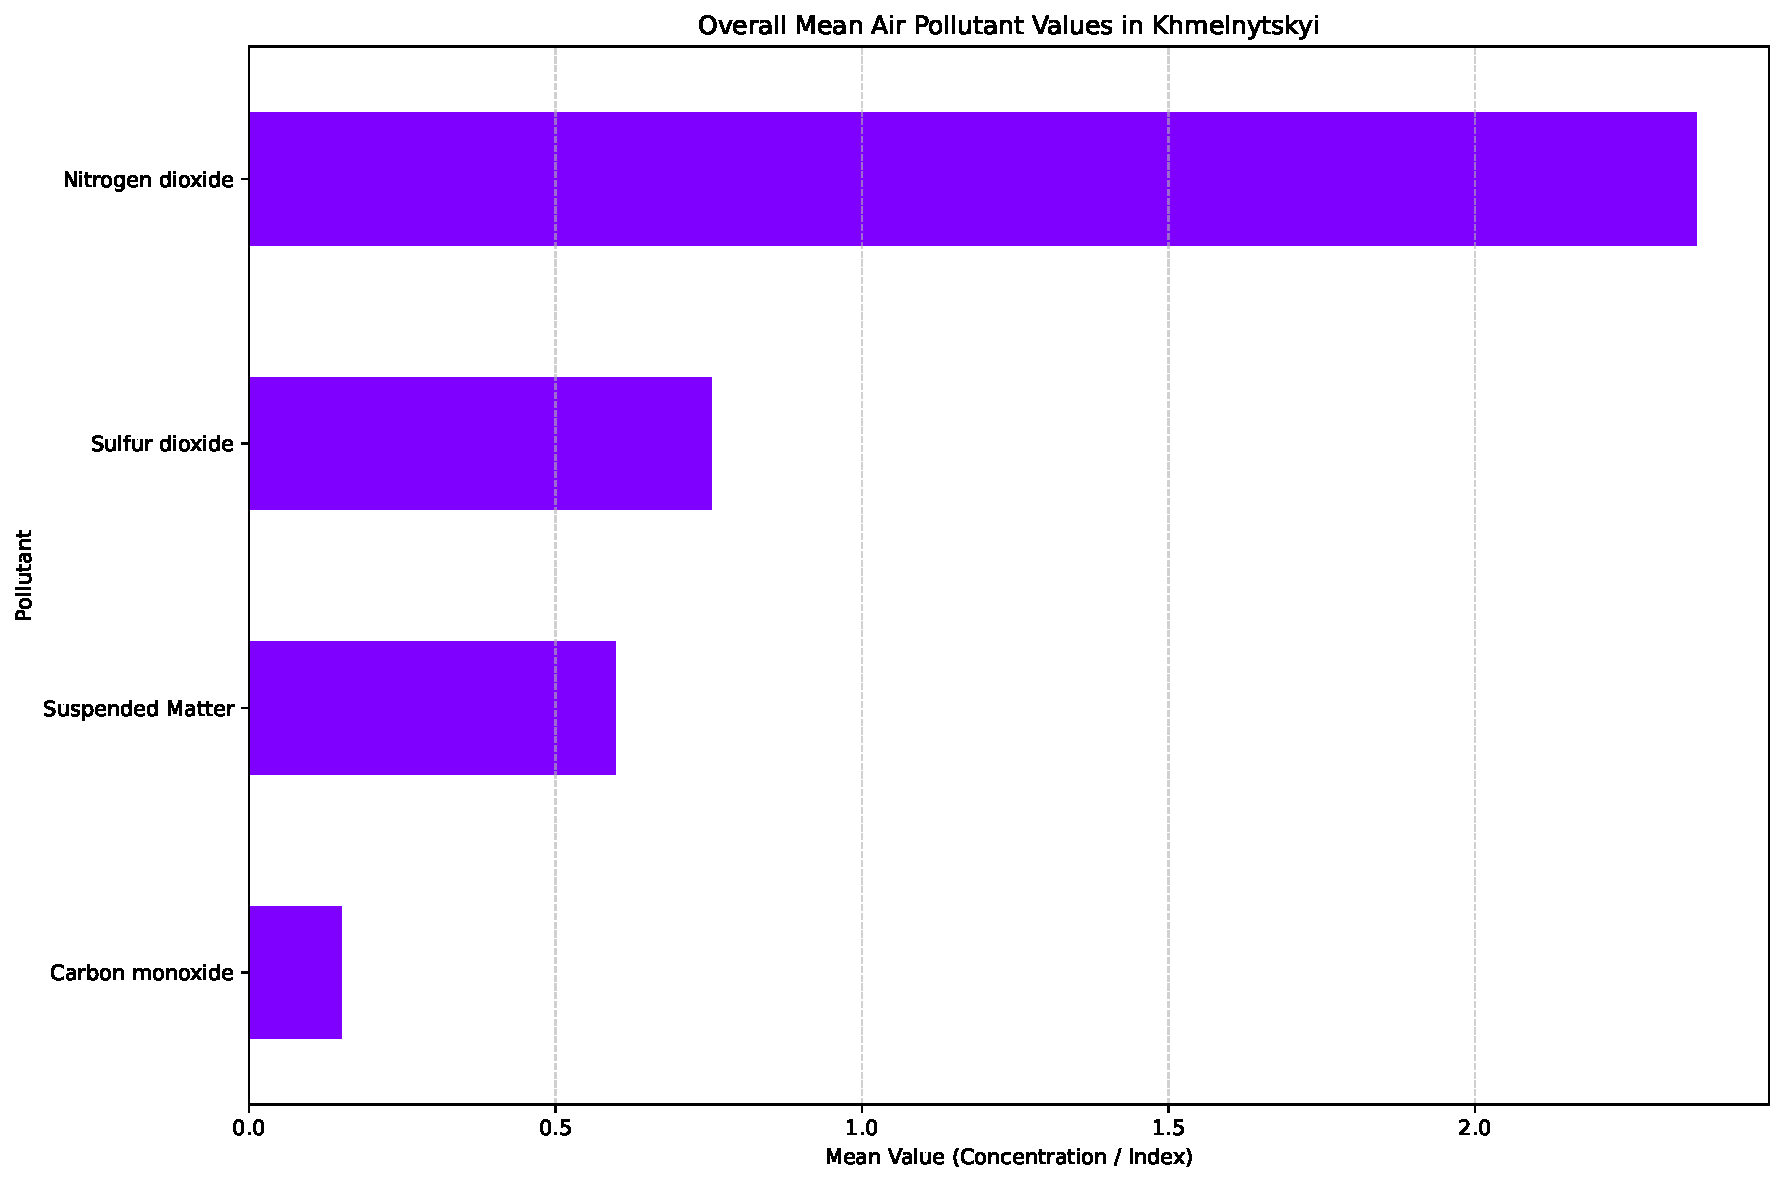
\includegraphics[width=\textwidth]{../plots/khmelnytskyi_stats_plots/overall_mean_by_pollutant.pdf}
\caption{Горизонтальний стовпчиковий графік середніх значень забруднюючих
речовин в Хмельницькому. Як бачимо, найбільш концентрованими забруднюючими
речовинами є nitrogen dioxide, formaldehyde та suspanded matter, які мають
найбільші середні значення серед усіх забруднюючих речовин. Це може свідчити про
наявність промислових викидів або інших джерел забруднення, які потребують
додаткового дослідження.}
\label{fig:overall_means}
\end{figure}

\subsubsection{Показники по роках}

Також можна відобразити показники по роках для кожної забруднюючої речовини, щоб
побачити, як змінюється рівень забруднення протягом часу. Для цього ми зобразимо
\textit{box plot} – графік, що показує середнє значення, 1-3 квантиль, а також
min/max значення. Він побудований для кожної забруднюючої речовини за допомогою 
наступного коду на Python:
\begin{minted}{python}
def plot_yearly_distributions(df, pollutant_columns, output_dir="plots/yearly_comparison"):
    """
    Generates and saves box plots showing the distribution of each pollutant
    level for each year.
    """
    
    print("\nGenerating yearly distribution box plots...")
    output_path = Path(output_dir)
    output_path.mkdir(parents=True, exist_ok=True)
    print(f"Ensured directory exists: {output_path}")

    df_with_year = df.copy()
    df_with_year.index = pd.to_datetime(df_with_year.index)
    df_with_year = df_with_year[df_with_year.index.notna()]
    df_with_year['Year'] = df_with_year.index.year

    for col in pollutant_columns:
        plt.figure(figsize=(12, 7))

        if col not in df_with_year or df_with_year[col].isnull().all():
            print(f"No data for pollutant '{col}'. Skipping yearly box plot.")
            plt.close()
            continue

        # Again, setting some styles and stuff
        sns.boxplot(x='Year', y=col, data=df_with_year, palette="viridis")
        plt.title(f'Yearly Distribution of {col}', fontsize=16)
        plt.xlabel('Year', fontsize=12)
        plt.ylabel(f'{col} Level', fontsize=12)
        plt.grid(axis='y', linestyle='--', alpha=0.6)
        plt.tight_layout()

        safe_col_name = col.replace(' ', '_').replace('/', '_').lower()
        full_plot_path = output_path / f"boxplot_yearly_{safe_col_name}.pdf"

        try:
            plt.savefig(full_plot_path, dpi=300, format='pdf', bbox_inches='tight')
            print(f"Saved yearly box plot to: {full_plot_path}")
        except Exception as e:
            print(f"Error saving box plot for {col}: {e}")

        plt.close()
\end{minted}

Результати зображено на Рисунку~\ref{fig:yearly_boxplots}.
\begin{figure}
    \begin{tabular}{ccc}
      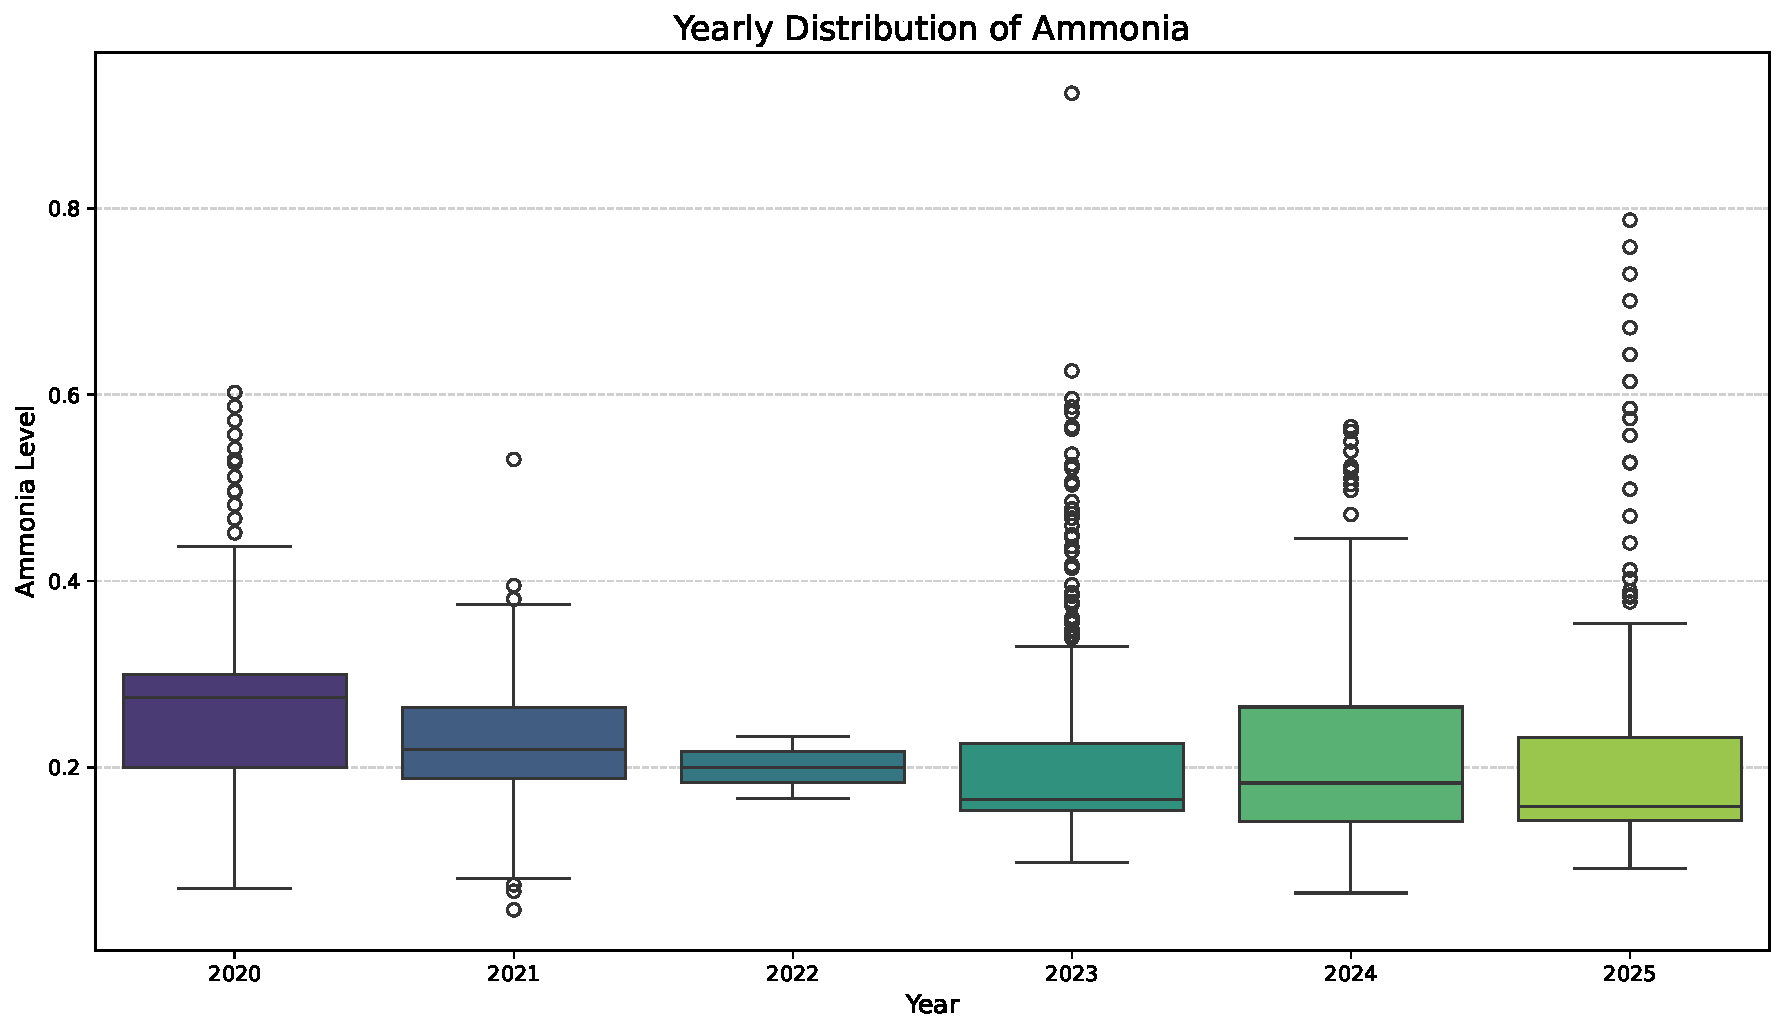
\includegraphics[width=0.33\textwidth]{../plots/khmelnytskyi_stats_plots/yearly_comparison/boxplot_yearly_ammonia.pdf} & 
      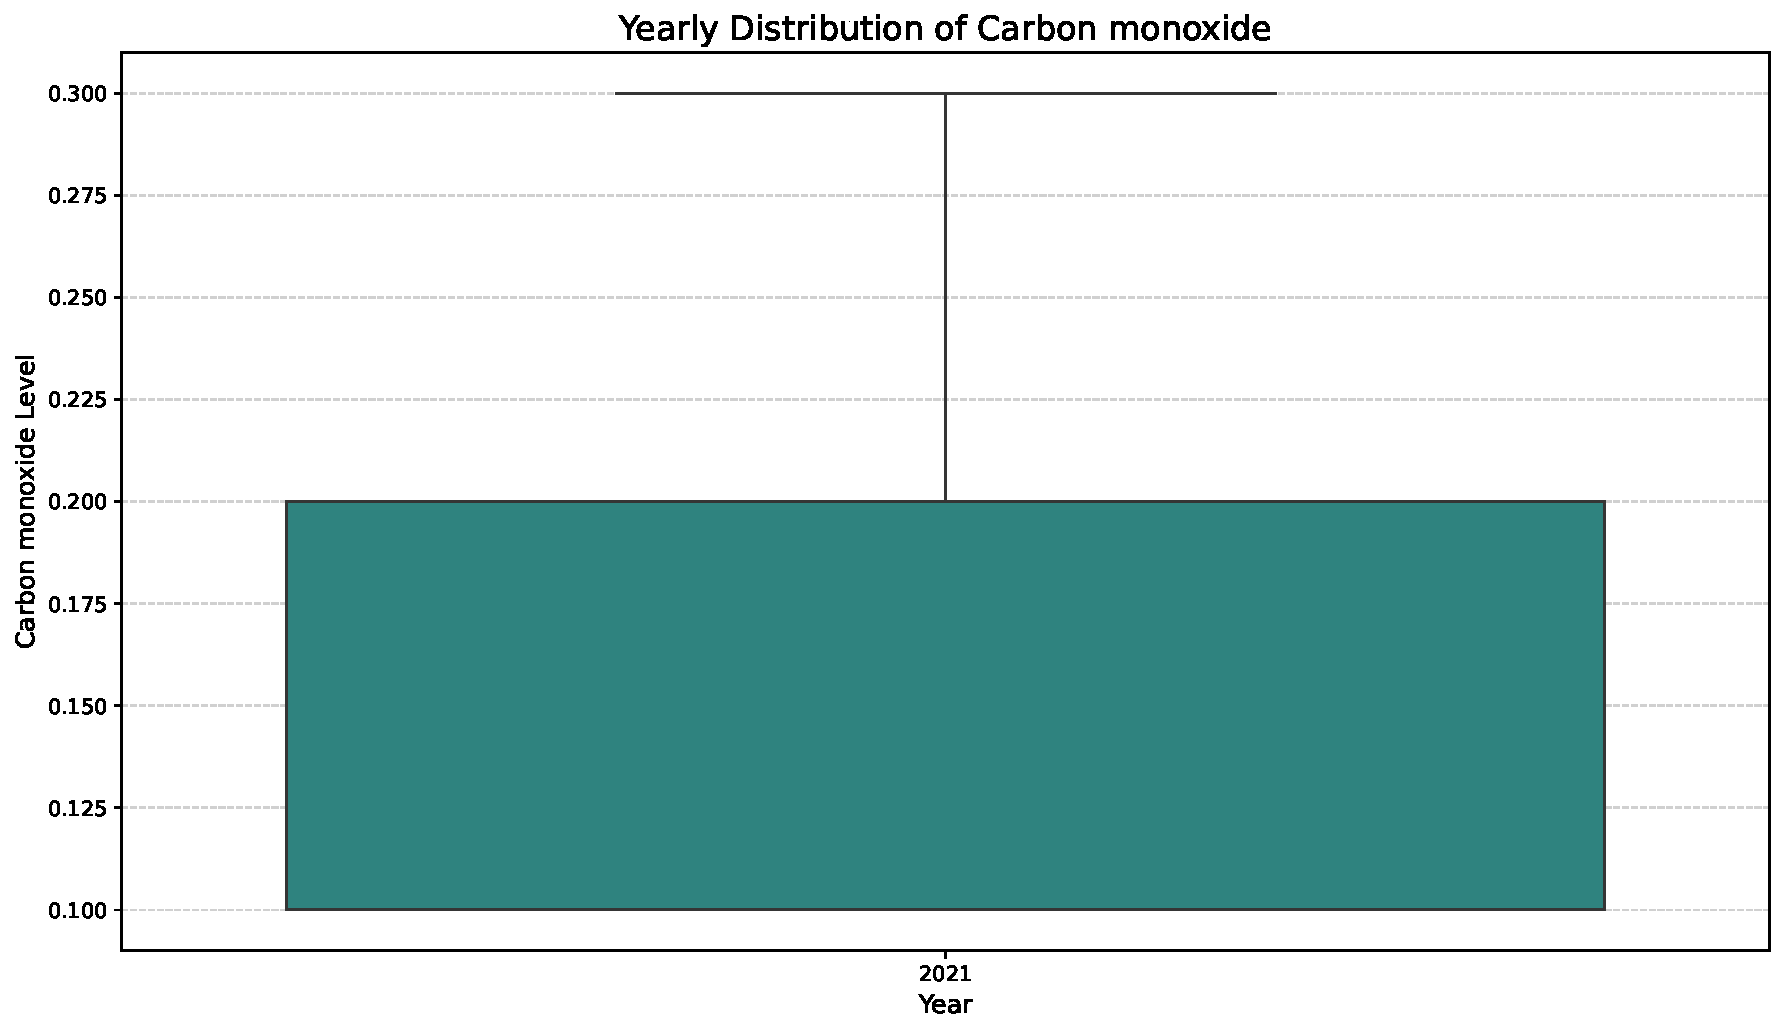
\includegraphics[width=0.33\textwidth]{../plots/khmelnytskyi_stats_plots/yearly_comparison/boxplot_yearly_carbon_monoxide.pdf} &
      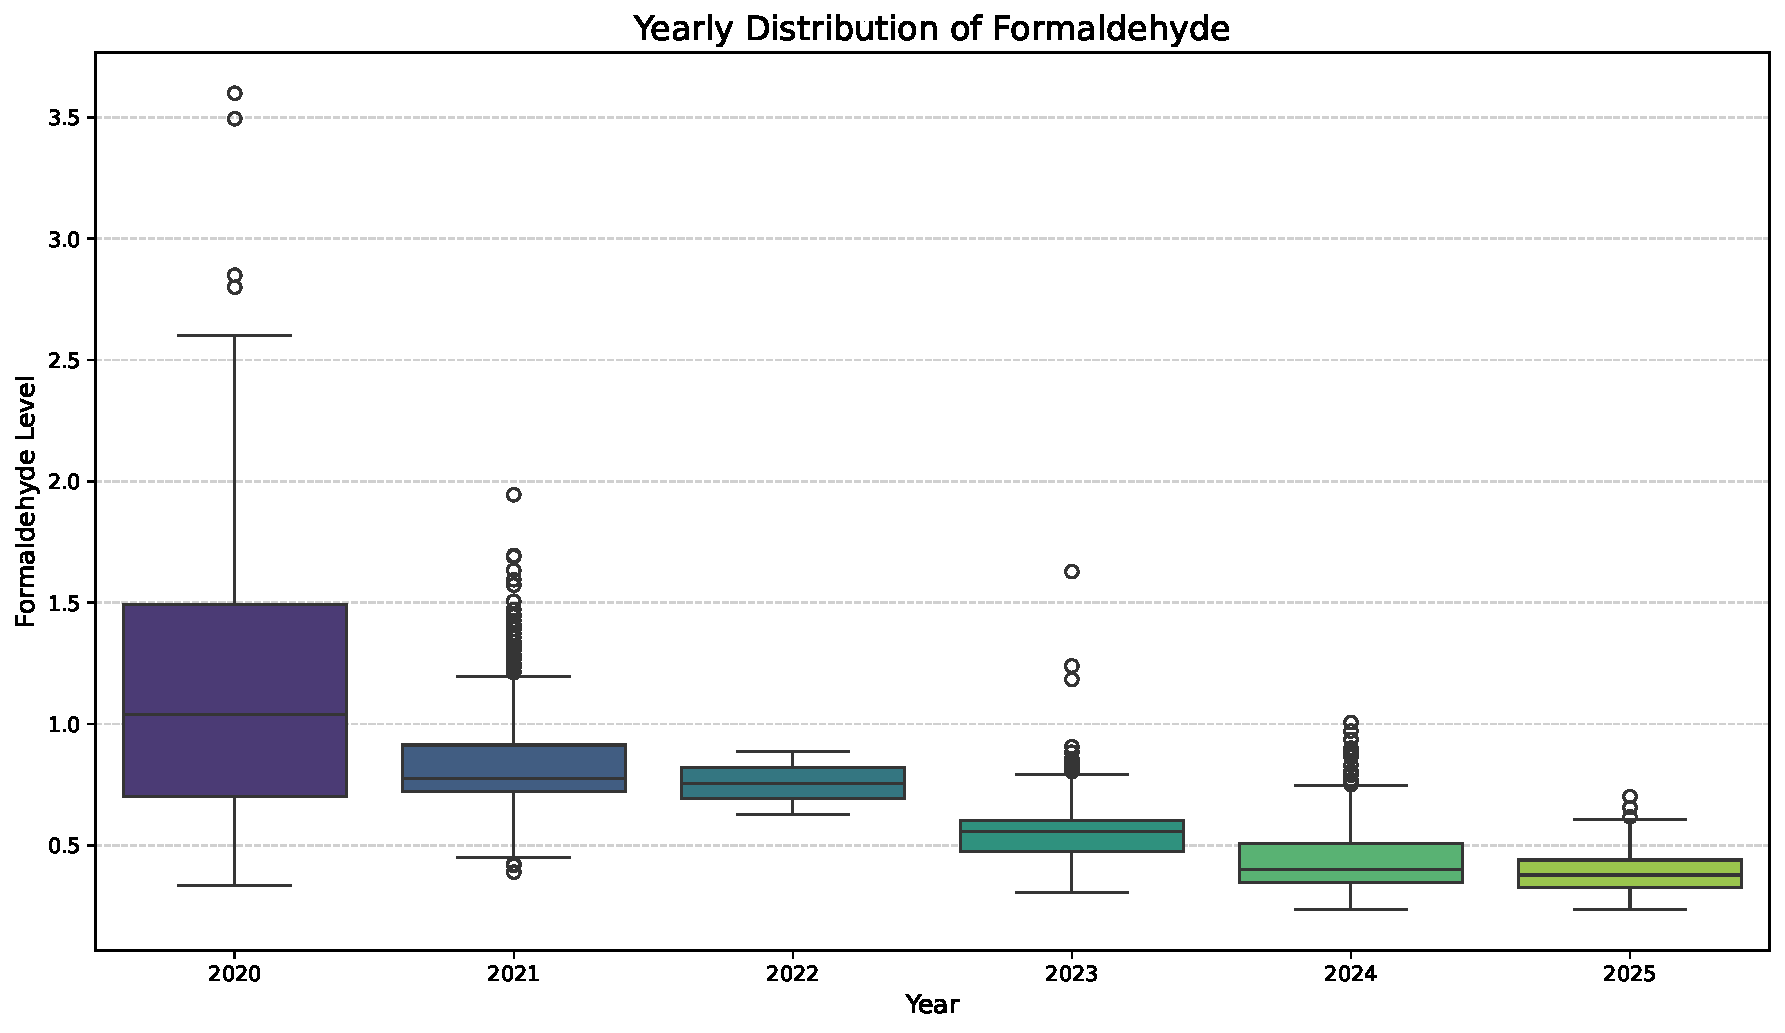
\includegraphics[width=0.33\textwidth]{../plots/khmelnytskyi_stats_plots/yearly_comparison/boxplot_yearly_formaldehyde.pdf} \\
      Ammonia & Carbon Monoxide & Formaldehyde \\
      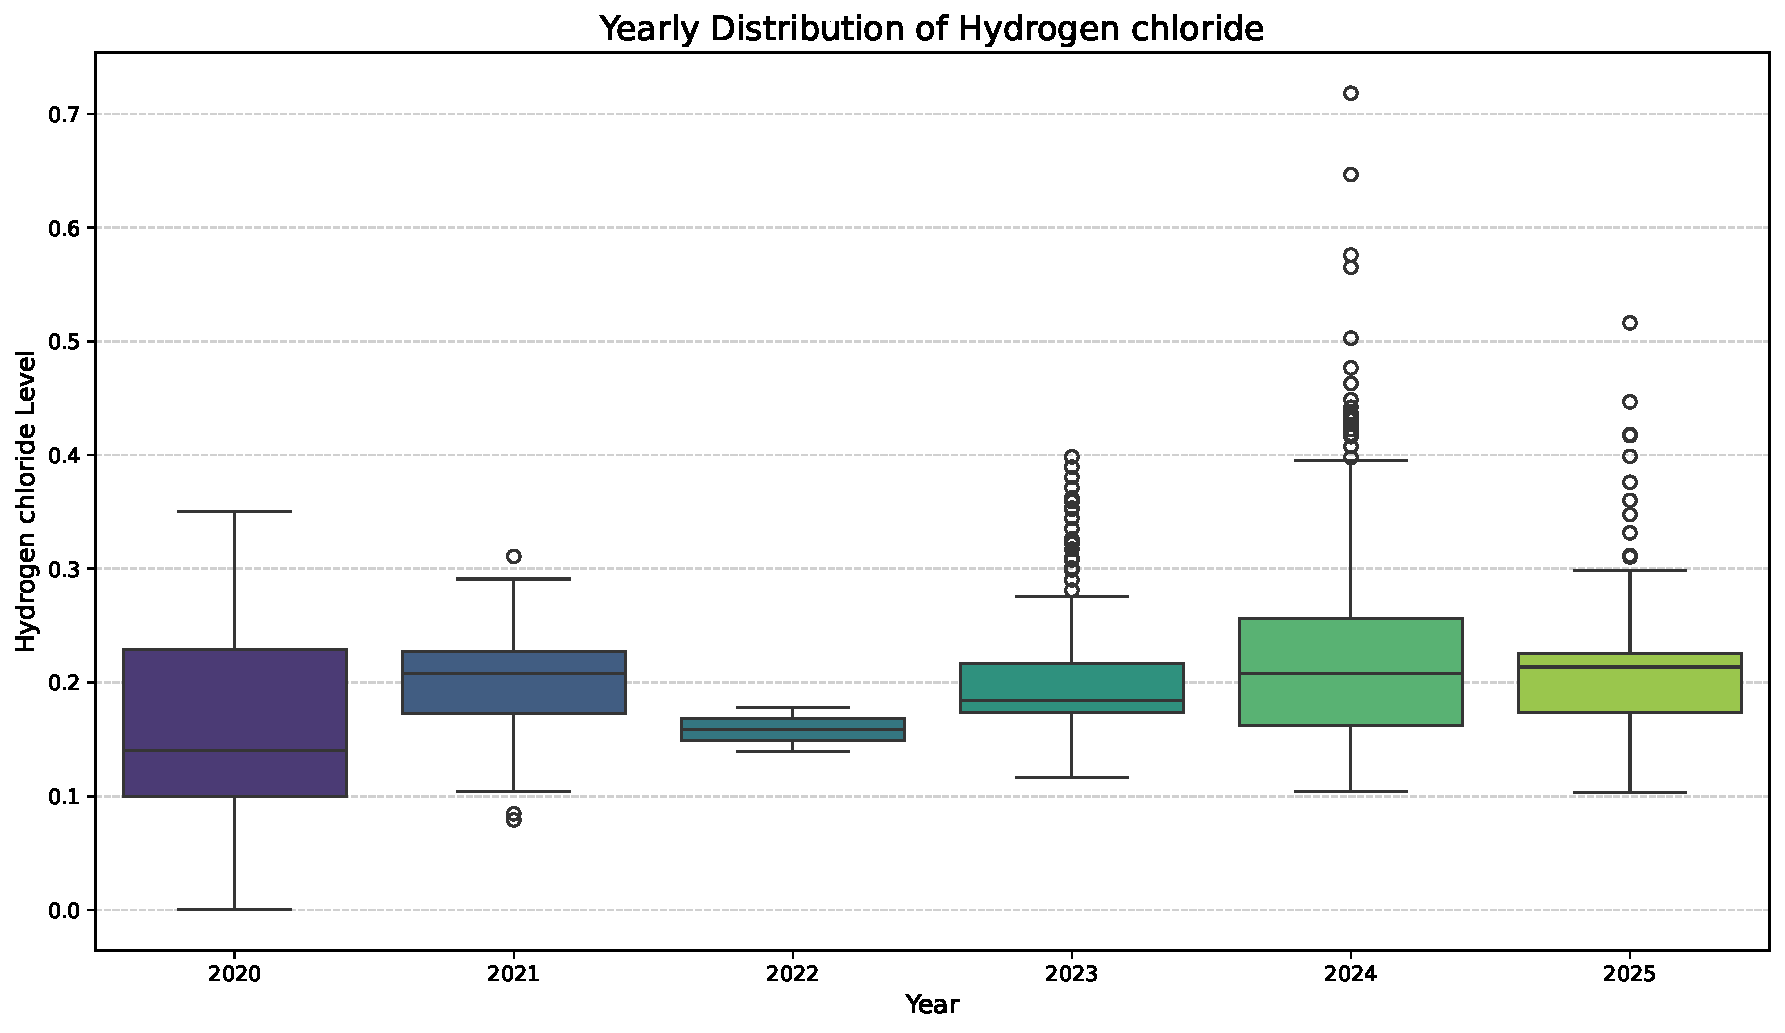
\includegraphics[width=0.33\textwidth]{../plots/khmelnytskyi_stats_plots/yearly_comparison/boxplot_yearly_hydrogen_chloride.pdf} &
      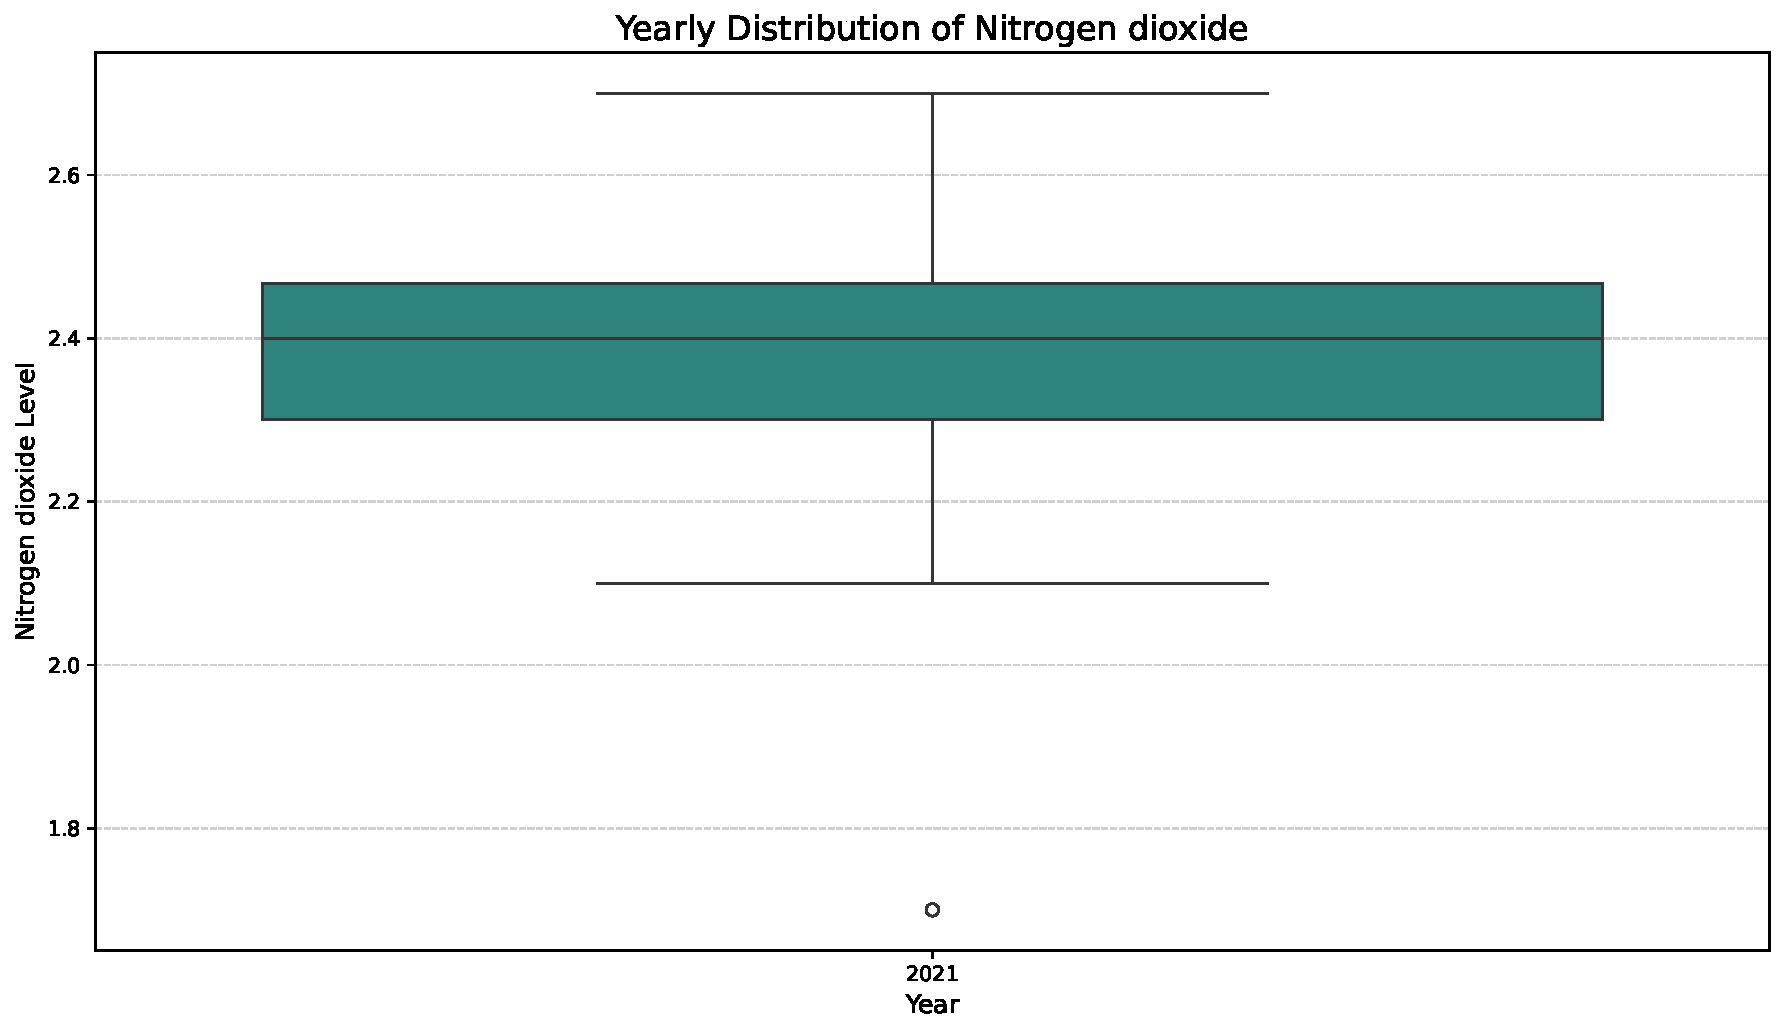
\includegraphics[width=0.33\textwidth]{../plots/khmelnytskyi_stats_plots/yearly_comparison/boxplot_yearly_nitrogen_dioxide.pdf} &
      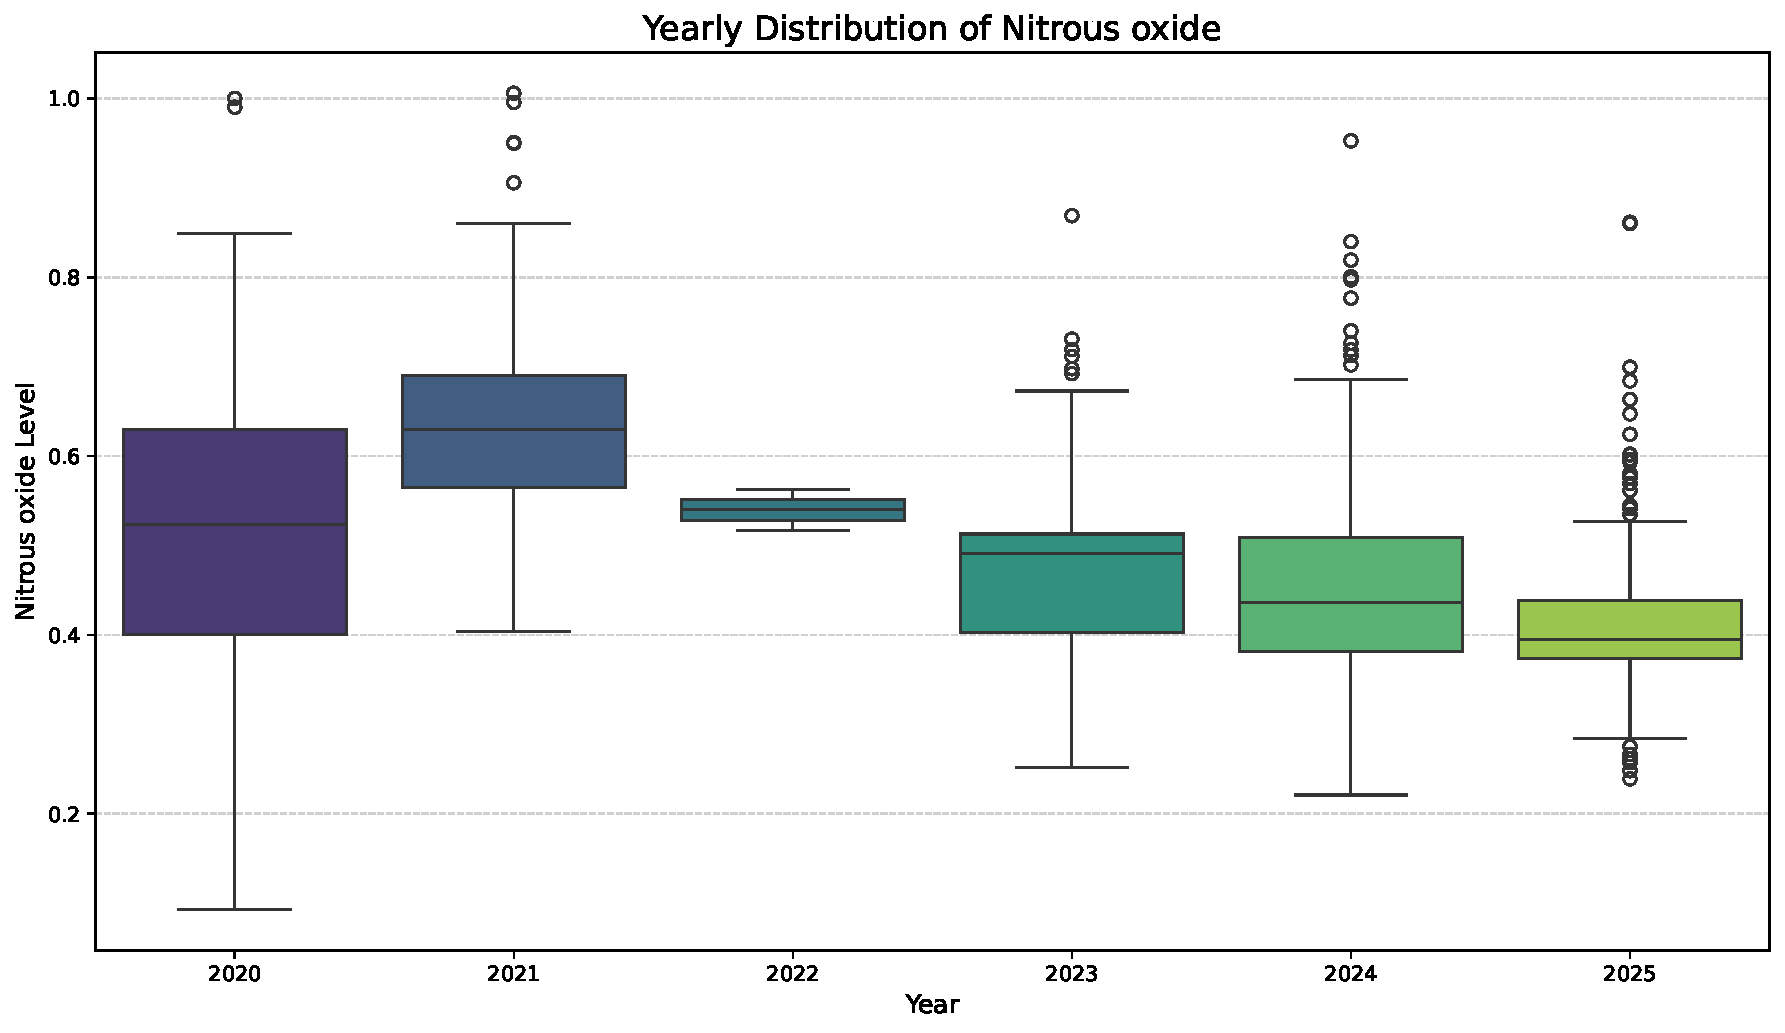
\includegraphics[width=0.33\textwidth]{../plots/khmelnytskyi_stats_plots/yearly_comparison/boxplot_yearly_nitrous_oxide.pdf} \\
        Hydrogen Chloride & Nitrogen Dioxide & Nitrous Oxide \\
      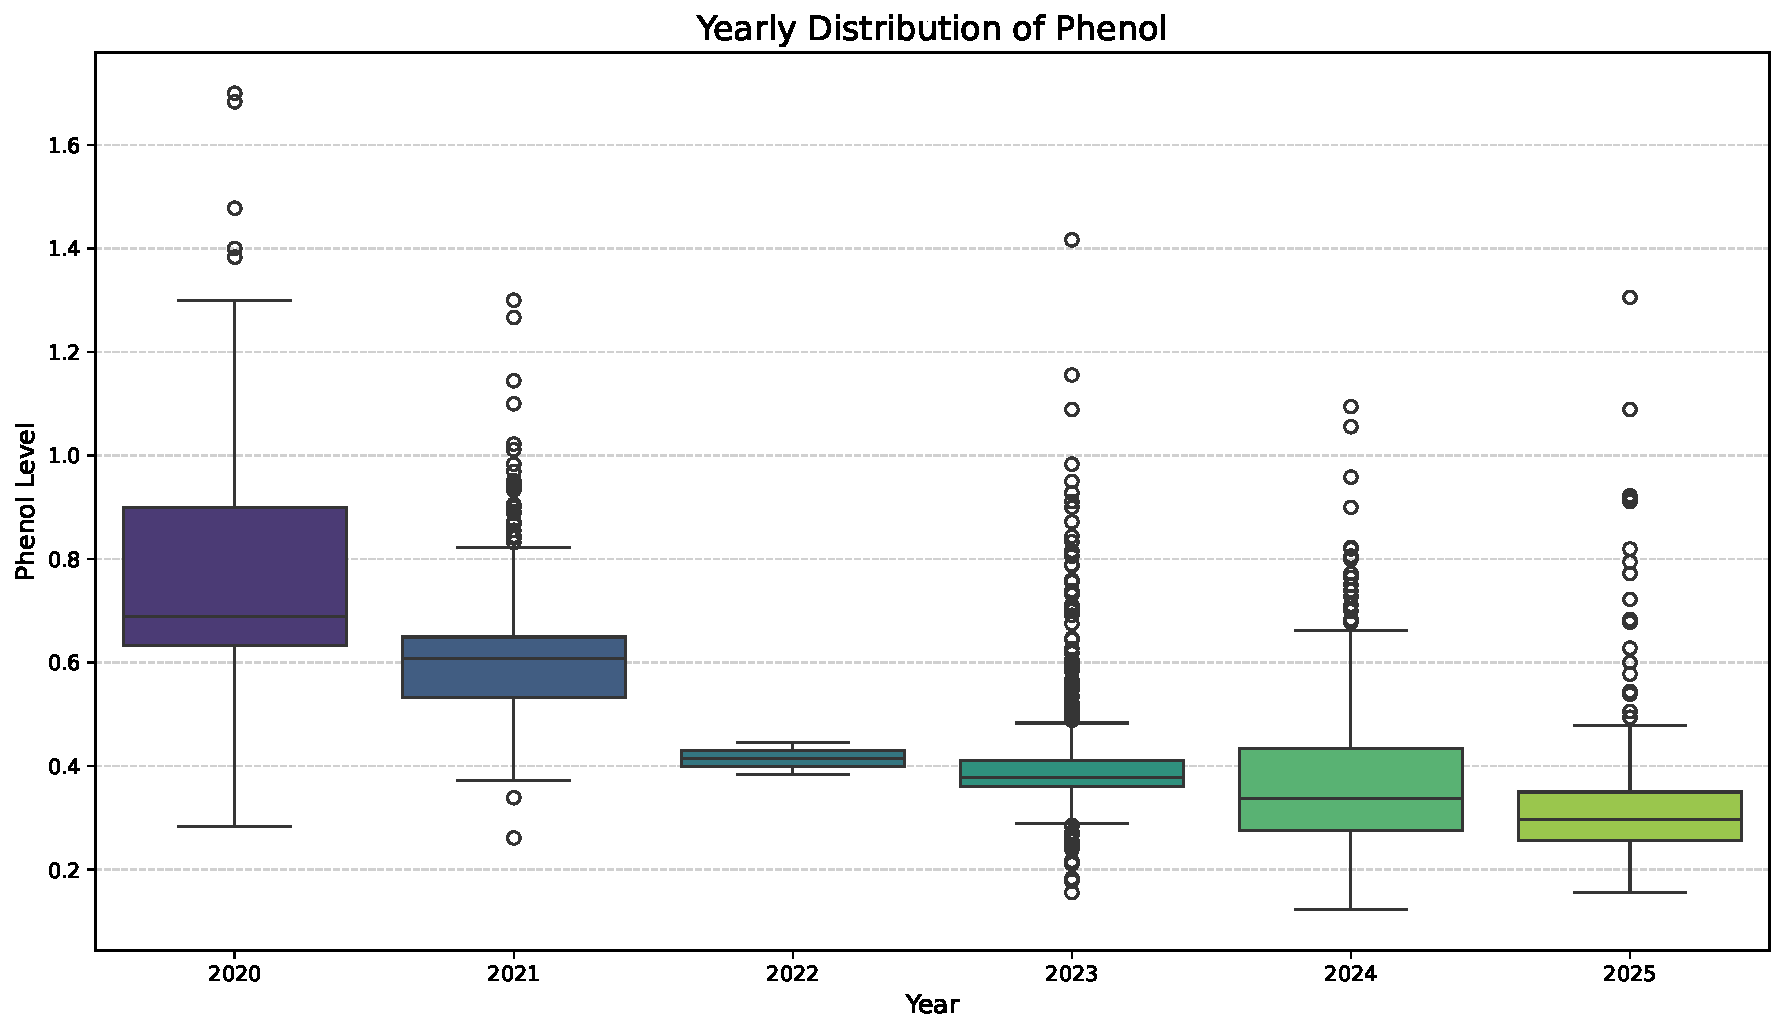
\includegraphics[width=0.33\textwidth]{../plots/khmelnytskyi_stats_plots/yearly_comparison/boxplot_yearly_phenol.pdf} &
      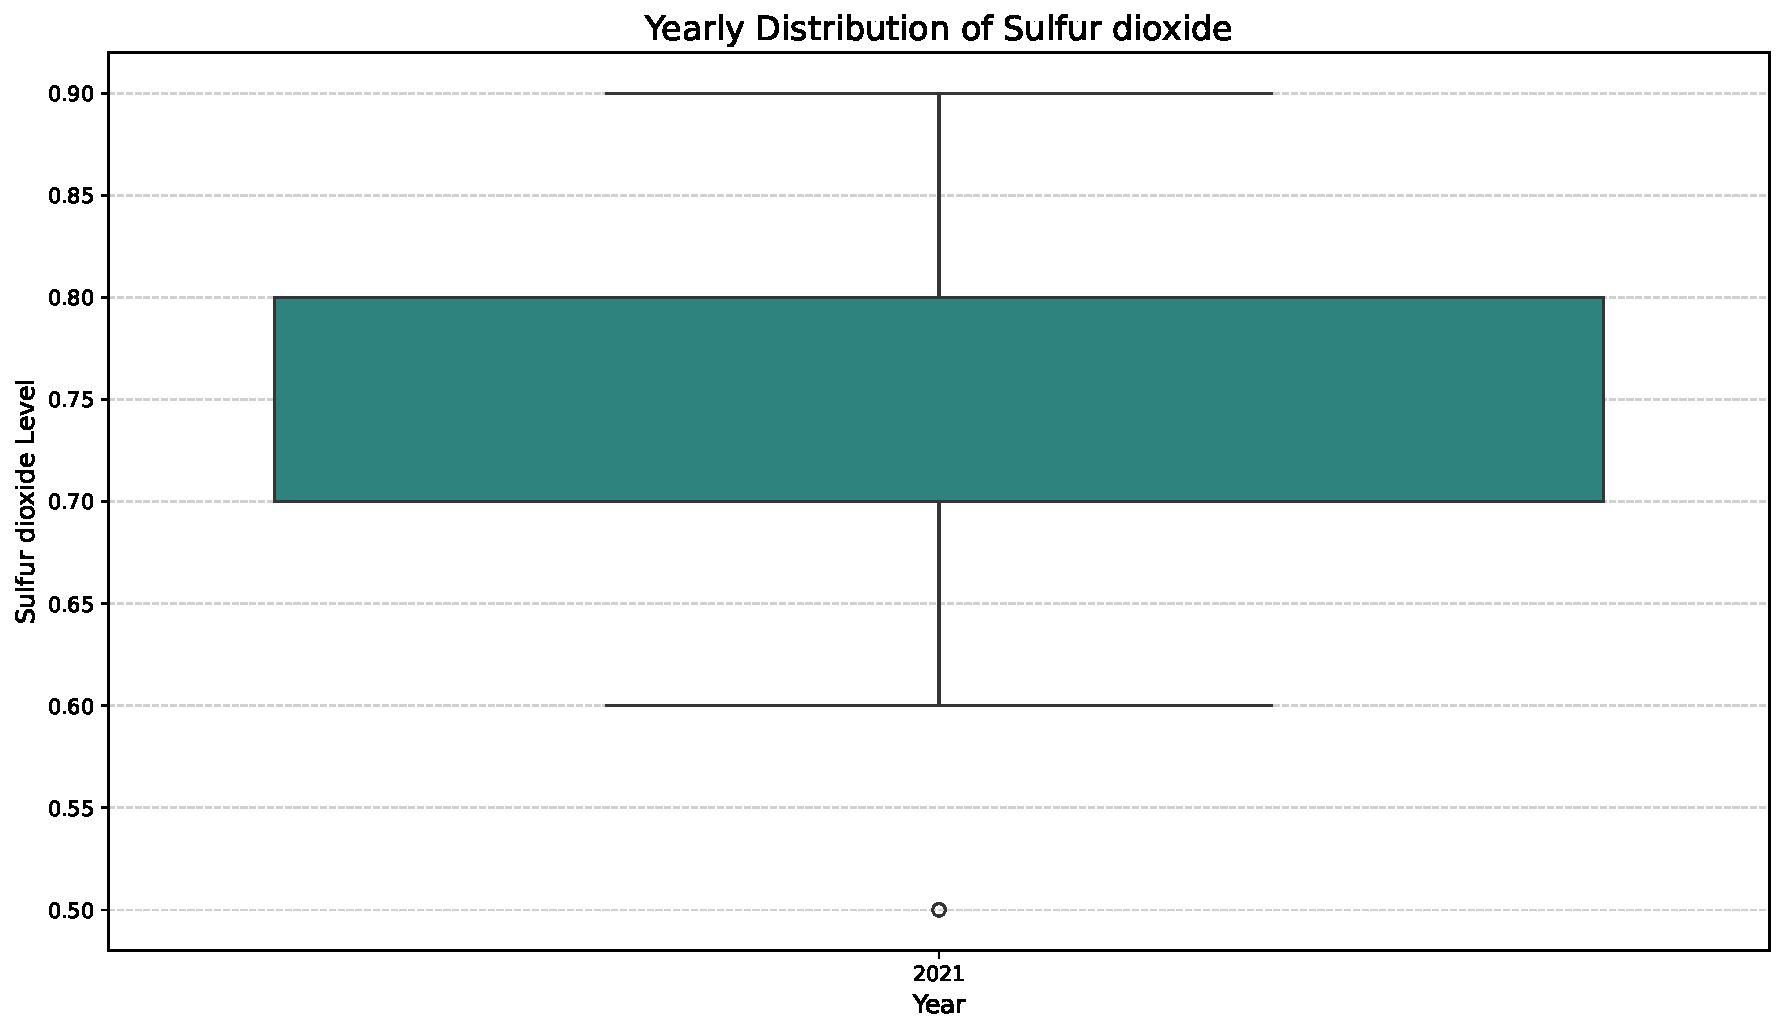
\includegraphics[width=0.33\textwidth]{../plots/khmelnytskyi_stats_plots/yearly_comparison/boxplot_yearly_sulfur_dioxide.pdf} &
      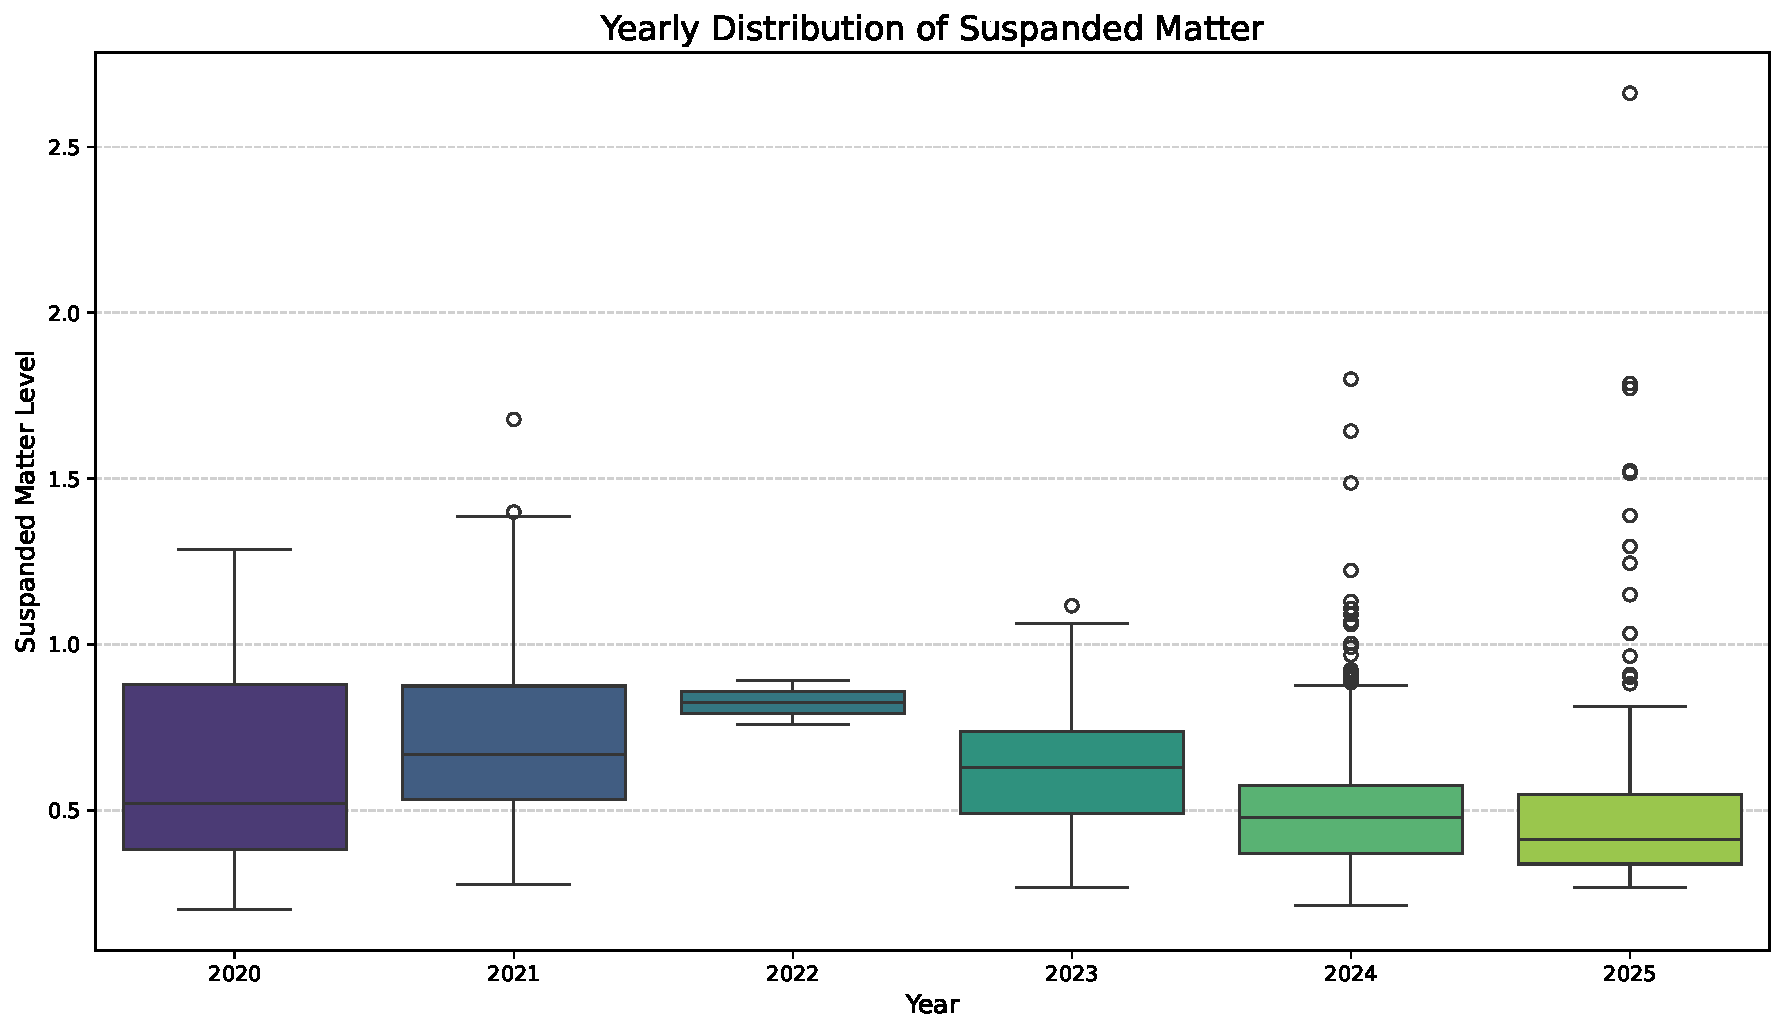
\includegraphics[width=0.33\textwidth]{../plots/khmelnytskyi_stats_plots/yearly_comparison/boxplot_yearly_suspanded_matter.pdf} \\
        Phenol & Sulfur Dioxide & Suspended Matter \\
    \end{tabular}
    \caption{\textit{Box plot} для кожної забруднюючої речовини по роках.}
    \label{fig:yearly_boxplots}
\end{figure}

\subsection{Спектральний аналіз}

Якщо нам наданий набір даних $X_1,\dots,X_n$, то дискретне перетворення Фур'є
(DFT) визначається як набір наступних комплексних чисел: 
\begin{equation*}
    \widehat{X}_k = \sum_{j \in [n]}X_je^{-2\pi ijk/n}, \quad k \in [n],
\end{equation*} 
де через $[n]$ ми позначили $\{0,\dots,n-1\}$. Ці числа є коефіцієнтами Фур'є,
які містить інформацію про частотний склад компоненти $\frac{k}{n}$. Амплітуда 
та фаза кожного коефіцієнта Фур'є визначаються як:
\begin{equation*}
    A_k = \frac{2|\widehat{X}_k|}{n}, \quad \phi_k = \arg(\widehat{X}_k).
\end{equation*}

Амплітудний спектр в такому разі будується як набір пар $\{\left(\frac{k}{n},
A_k\right)\}_{k \in [n]}$, а відповідно фазовий спектр як набір пар
$\{\left(\frac{k}{n}, \phi_k\right)\}_{k \in [n]}$. Висока амплітуда буде
показувати на що, що в даних присутня сильна гармоніка $\frac{k}{n}$, а фаза
показує початковий зсув цієї гармоніки. Напишемо код для цього:
\begin{minted}{python}
DEFAULT_NUM_HARMONICS: int = 9  # Default number of harmonics to analyze


def perform_fft_analysis(df, pollutant_columns, num_harmonics: int = DEFAULT_NUM_HARMONICS):
    """
    Performs FFT on each pollutant time series to find amplitudes and phases
    of the first N harmonics (excluding the 0th component).
    """
    
    results = {}

    print(f"Performing FFT for first {num_harmonics} harmonics...")

    for col in pollutant_columns:
        data_series = df[col].dropna()
        N = len(data_series)

        # Check if there's enough data
        if N < (num_harmonics + 1) * 2: # Need at least ~2 points per harmonic
            print(f"Warning: Not enough data for {col} ({N} points). Skipping FFT.")
            continue

        try:
            # Perform FFT
            yf = np.fft.fft(data_series.values)

            # Calculate amplitudes and phases for the first N harmonics (indices 1 to N)
            # Amplitude = 2.0/N * |Y(f)| for f > 0
            amplitudes = 2.0 / N * np.abs(yf[1 : num_harmonics + 1])
            phases = np.angle(yf[1 : num_harmonics + 1]) # Phase in radians

            results[col] = {'Amplitude': amplitudes, 'Phase': phases}

        except Exception as e:
            print(f"Error performing FFT for {col}: {e}")
            continue

    if not results:
        print("FFT analysis failed for all pollutants.")
        return None, None

    # Convert results to DataFrames for easier plotting
    amp_df = pd.DataFrame({k: v['Amplitude'] for k, v in results.items()})
    phase_df = pd.DataFrame({k: v['Phase'] for k, v in results.items()})

    # Set index to '1' through 'num_harmonics'
    harmonic_index = range(1, num_harmonics + 1)
    amp_df.index = harmonic_index
    phase_df.index = harmonic_index
    amp_df.index.name = "Harmonic"
    phase_df.index.name = "Harmonic"

    print("FFT analysis complete.")
    return amp_df, phase_df
\end{minted}

Результати перетворення Фур'є для кожної забруднюючої речовини 
збережено в CSV-файли \texttt{fft\_amplitudes.csv} та
\texttt{fft\_phases.csv}. Візуалізуємо ці результати 
за допомогою наступного коду на Python:
\begin{minted}{python}
def _plot_spectrum_bars(spec_df, title, ylabel, filename, output_dir):
    """
    Helper function to plot amplitude or phase spectrum as a grouped bar plot.
    """
    
    if spec_df is None or spec_df.empty:
        print(f"No spectrum data provided for {title}. Skipping plot.")
        return

    output_path = Path(output_dir)
    output_path.mkdir(parents=True, exist_ok=True)

    num_harmonics, num_pollutants = spec_df.shape
    fig_width = max(12, num_harmonics * num_pollutants * 0.2)

    _ = spec_df.plot(kind='bar', figsize=(fig_width, 7), width=0.8)

    plt.title(title, fontsize=16)
    plt.xlabel('Harmonic Index (Frequency Component)', fontsize=12)
    plt.ylabel(ylabel, fontsize=12)
    plt.xticks(rotation=0)
    plt.legend(title='Pollutants', bbox_to_anchor=(1.02, 1), loc='upper left')
    plt.grid(axis='y', linestyle='--', alpha=0.7)
    plt.tight_layout(rect=[0, 0, 0.88, 1])

    full_plot_path = output_path / f"{filename}.pdf"

    try:
        plt.savefig(full_plot_path, dpi=300, format='pdf', bbox_inches='tight')
        plt.close()
        print(f"Saved spectrum plot to: {full_plot_path}")
    except Exception as e:
        print(f"Error saving spectrum plot {full_plot_path}: {e}")


def plot_amplitude_spectrum(amp_df, output_dir="plots"):
    """
    Plots the amplitude spectrum as a grouped bar plot.
    """
    
    _plot_spectrum_bars(amp_df,
                        'Amplitude Spectrum of Pollutant Oscillations',
                        'Amplitude',
                        'amplitude_spectrum',
                        output_dir)


def plot_phase_spectrum(phase_df, output_dir="plots"):
    """
    Plots the phase spectrum as a grouped bar plot.
    """
    
    _plot_spectrum_bars(phase_df,
                        'Phase Spectrum of Pollutant Oscillations',
                        'Phase (Radians)',
                        'phase_spectrum',
                        output_dir)
\end{minted}

Результати спектрального аналізу зображено на Рисунку~\ref{fig:fft_spectrum}.
\begin{figure}[H]
\centering
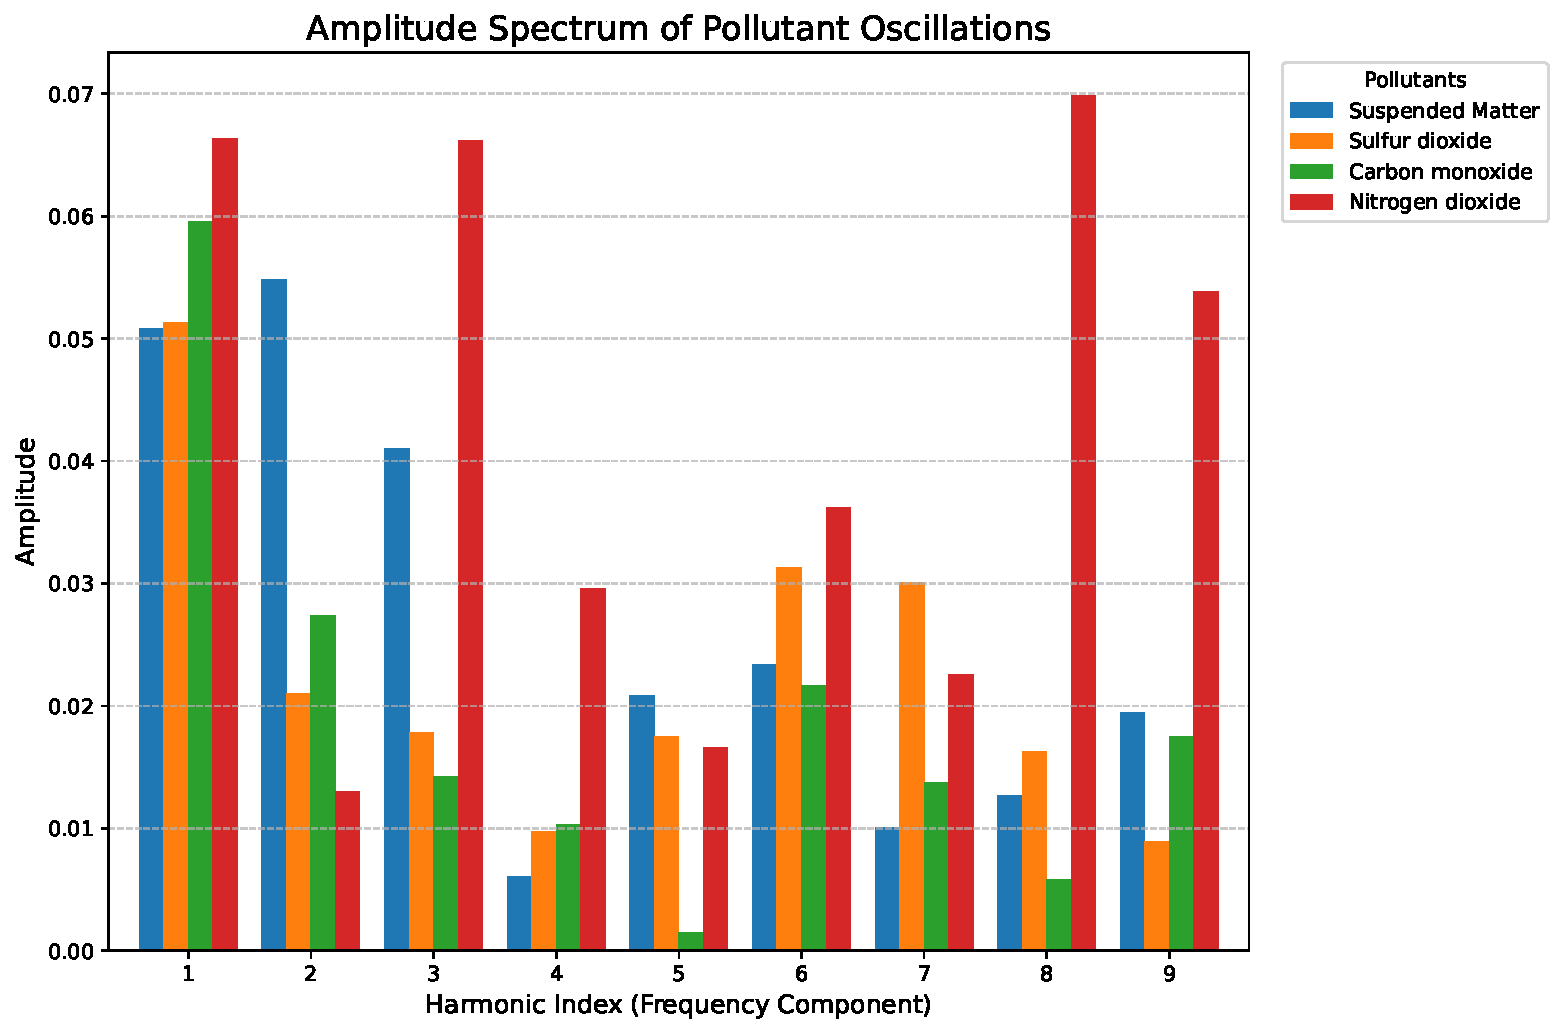
\includegraphics[width=\textwidth]{../plots/khmelnytskyi_stats_plots/spectrum_analysis/amplitude_spectrum.pdf}
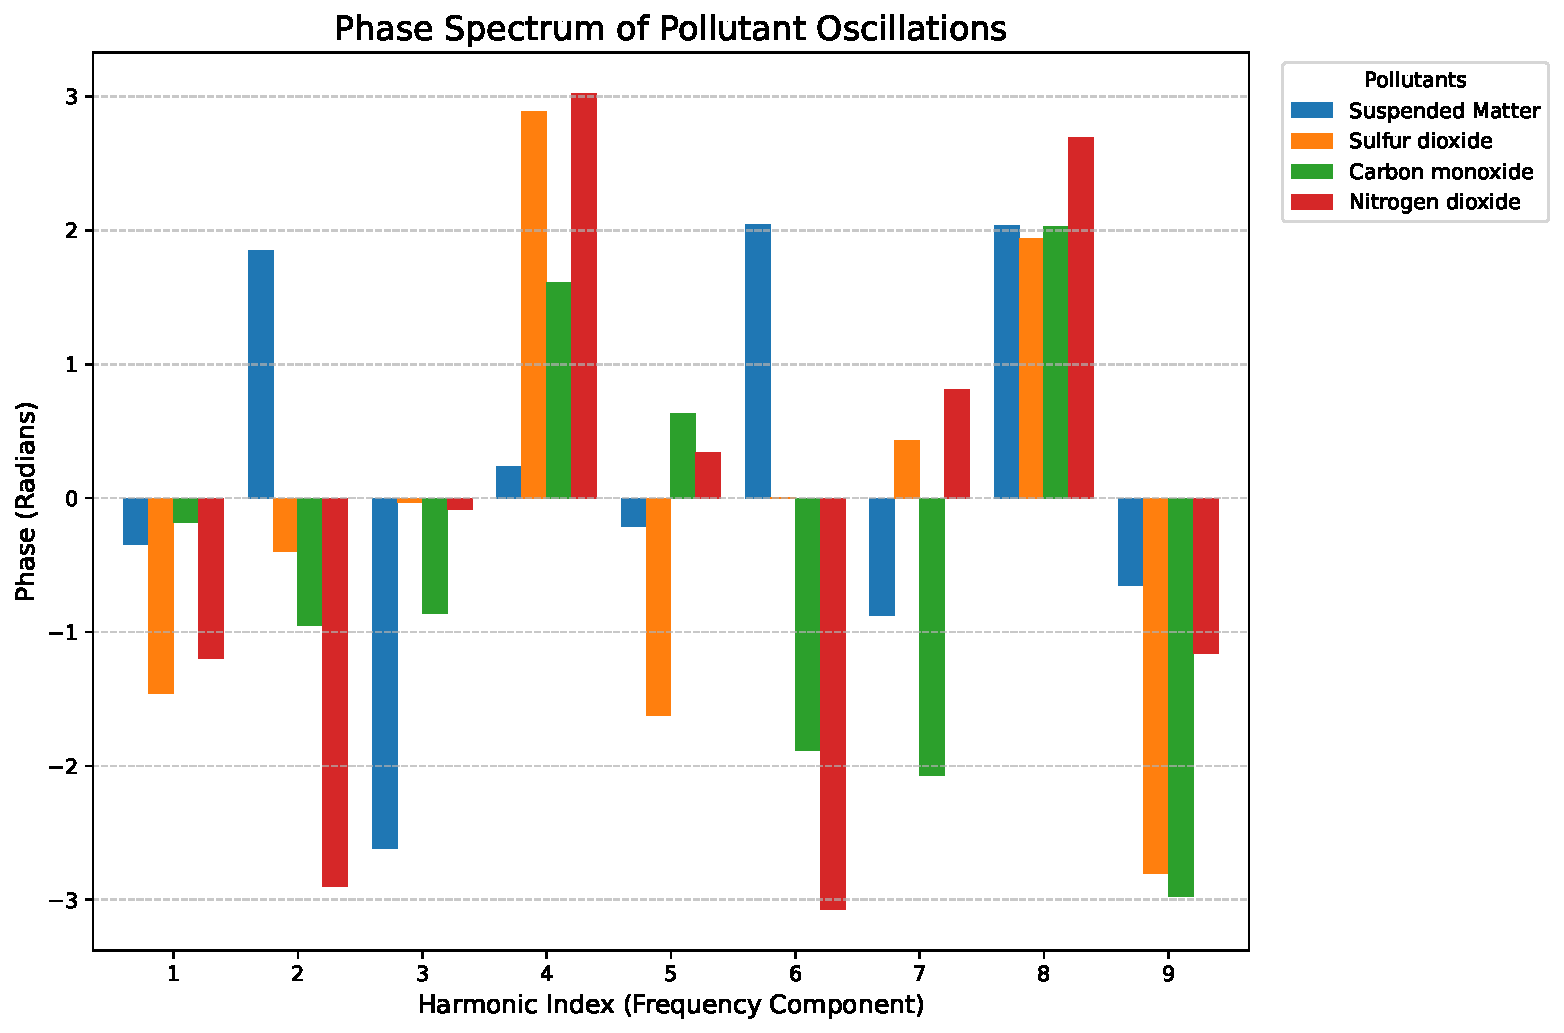
\includegraphics[width=\textwidth]{../plots/khmelnytskyi_stats_plots/spectrum_analysis/phase_spectrum.pdf}
\caption{Груповані стовпчикові графіки амплітудного та фазового спектрів
забруднюючих речовин в Хмельницькому.}
\label{fig:fft_spectrum}
\end{figure}

\subsection{Фазовий аналіз динамічної системи}

Щоб проаналізувати фазовий портрет забруднюючих речовин, ми можемо знайти
похідні від послідовних значень концентрації забруднюючих речовин та побудувати
графік залежності похідної від значення забруднюючої речовини (а також другої
похідної, за необхідності). Скажімо, якщо маємо значення $X_1,\dots,X_n$, то 
похідна $\dot{X}_i \approx \frac{X_{i+1}-X_{i-1}}{2\tau}$ де $\tau$ --- це
інтервал між послідовними значеннями. Другу похідну можна обрахувати як
$\ddot{X}_i \approx \frac{X_{i+1}-2X_i+X_{i-1}}{\tau^2}$. Обидві формули 
називаються \textbf{центральними різницями} і є наближеннями похідних для
дискретних даних. На щастя, в \texttt{pandas} вже є реалізовані 
методи для обрахунку похідних, тому ми можемо просто викликати їх на
даних. Маємо наступний код на Python:
\begin{minted}{python}
def plot_phase_analysis(
    df, 
    pollutant_columns, 
    output_dir="plots/phase_analysis"
) -> None:
    """
    Generates and saves phase analysis plots (derivatives vs. value/derivatives)
    for each pollutant in separate files.
    """
    
    if df.empty:
        print("DataFrame is empty. No phase plots will be generated.")
        return

    # Ensure the output directory exists
    output_path = Path(output_dir)
    output_path.mkdir(parents=True, exist_ok=True)
    print(f"Ensured directory exists: {output_path}")

    # Iterate through each pollutant column
    for col in pollutant_columns:
        # Calculate value and derivatives
        x = df[col]
        dx_dt = df[col].diff()  # 1st derivative (velocity)
        d2x_dt2 = dx_dt.diff() # 2nd derivative (acceleration)

        plot_df = pd.DataFrame({
            'x': x,
            'dx_dt': dx_dt,
            'd2x_dt2': d2x_dt2
        }).dropna()

        # Check if there is data left to plot
        if plot_df.empty:
            print(f"Not enough data (after differentiation) for {col}. Skipping phase plot.")
            continue
        
        # Save the derivative data to CSV
        safe_col_name = col.replace(' ', '_').replace('/', '_').lower()
        csv_filename = f"phase_data_{safe_col_name}.csv"
        full_csv_path = output_path / csv_filename
        try:
            plot_df.to_csv(full_csv_path)
            print(f"Saved phase derivative data for {col} to: {full_csv_path}")
        except Exception as e:
            print(f"Error saving phase data CSV for {col}: {e}")

        # Create a figure with 3 subplots for three phase portraits
        fig, axes = plt.subplots(1, 3, figsize=(20, 6)) # 1 row, 3 columns
        fig.suptitle(f'Phase Analysis Plots for {col}', fontsize=16, y=1.03)

        # Plot 1: 1st Der vs. Value (Velocity vs. Position)
        axes[0].scatter(plot_df['x'], plot_df['dx_dt'], s=5, alpha=0.3, color='blue')
        axes[0].set_title('1st Derivative vs. Value')
        axes[0].set_xlabel(f'{col} (Position)')
        axes[0].set_ylabel('1st Derivative (Velocity)')
        axes[0].grid(True, linestyle='--', alpha=0.6)

        # Plot 2: 2nd Der vs. Value (Acceleration vs. Position)
        axes[1].scatter(plot_df['x'], plot_df['d2x_dt2'], s=5, alpha=0.3, color='green')
        axes[1].set_title('2nd Derivative vs. Value')
        axes[1].set_xlabel(f'{col} (Position)')
        axes[1].set_ylabel('2nd Derivative (Acceleration)')
        axes[1].grid(True, linestyle='--', alpha=0.6)

        # Plot 3: 2nd Der vs. 1st Der (Phase Portrait)
        axes[2].scatter(plot_df['dx_dt'], plot_df['d2x_dt2'], s=5, alpha=0.3, color='red')
        axes[2].set_title('Phase Portrait (Acceleration vs. Velocity)')
        axes[2].set_xlabel('1st Derivative (Velocity)')
        axes[2].set_ylabel('2nd Derivative (Acceleration)')
        axes[2].grid(True, linestyle='--', alpha=0.6)

        plt.tight_layout(rect=[0, 0.03, 1, 0.98])

        # Prepare filename and save
        safe_col_name = col.replace(' ', '_').replace('/', '_').lower()
        plot_filename = f"phase_analysis_{safe_col_name}.pdf"
        full_plot_path = output_path / plot_filename

        try:
            plt.savefig(full_plot_path, dpi=300, format='pdf', bbox_inches='tight')
            print(f"Saved phase plot to: {full_plot_path}")
        except Exception as e:
            print(f"Error saving phase plot for {col}: {e}")

        plt.close(fig)
\end{minted}

Часткові результати фазового аналізу зображено на
Рисунку~\ref{fig:phase_analysis}. Для кожної забруднюючої речовини
ми побудували три портрети $(X, \dot{X})$, $(X, \ddot{X})$ та
$(\dot{X}, \ddot{X})$, де $X=X(t)$ --- це значення забруднюючої речовини 
як функція часу.

\begin{figure}
\centering
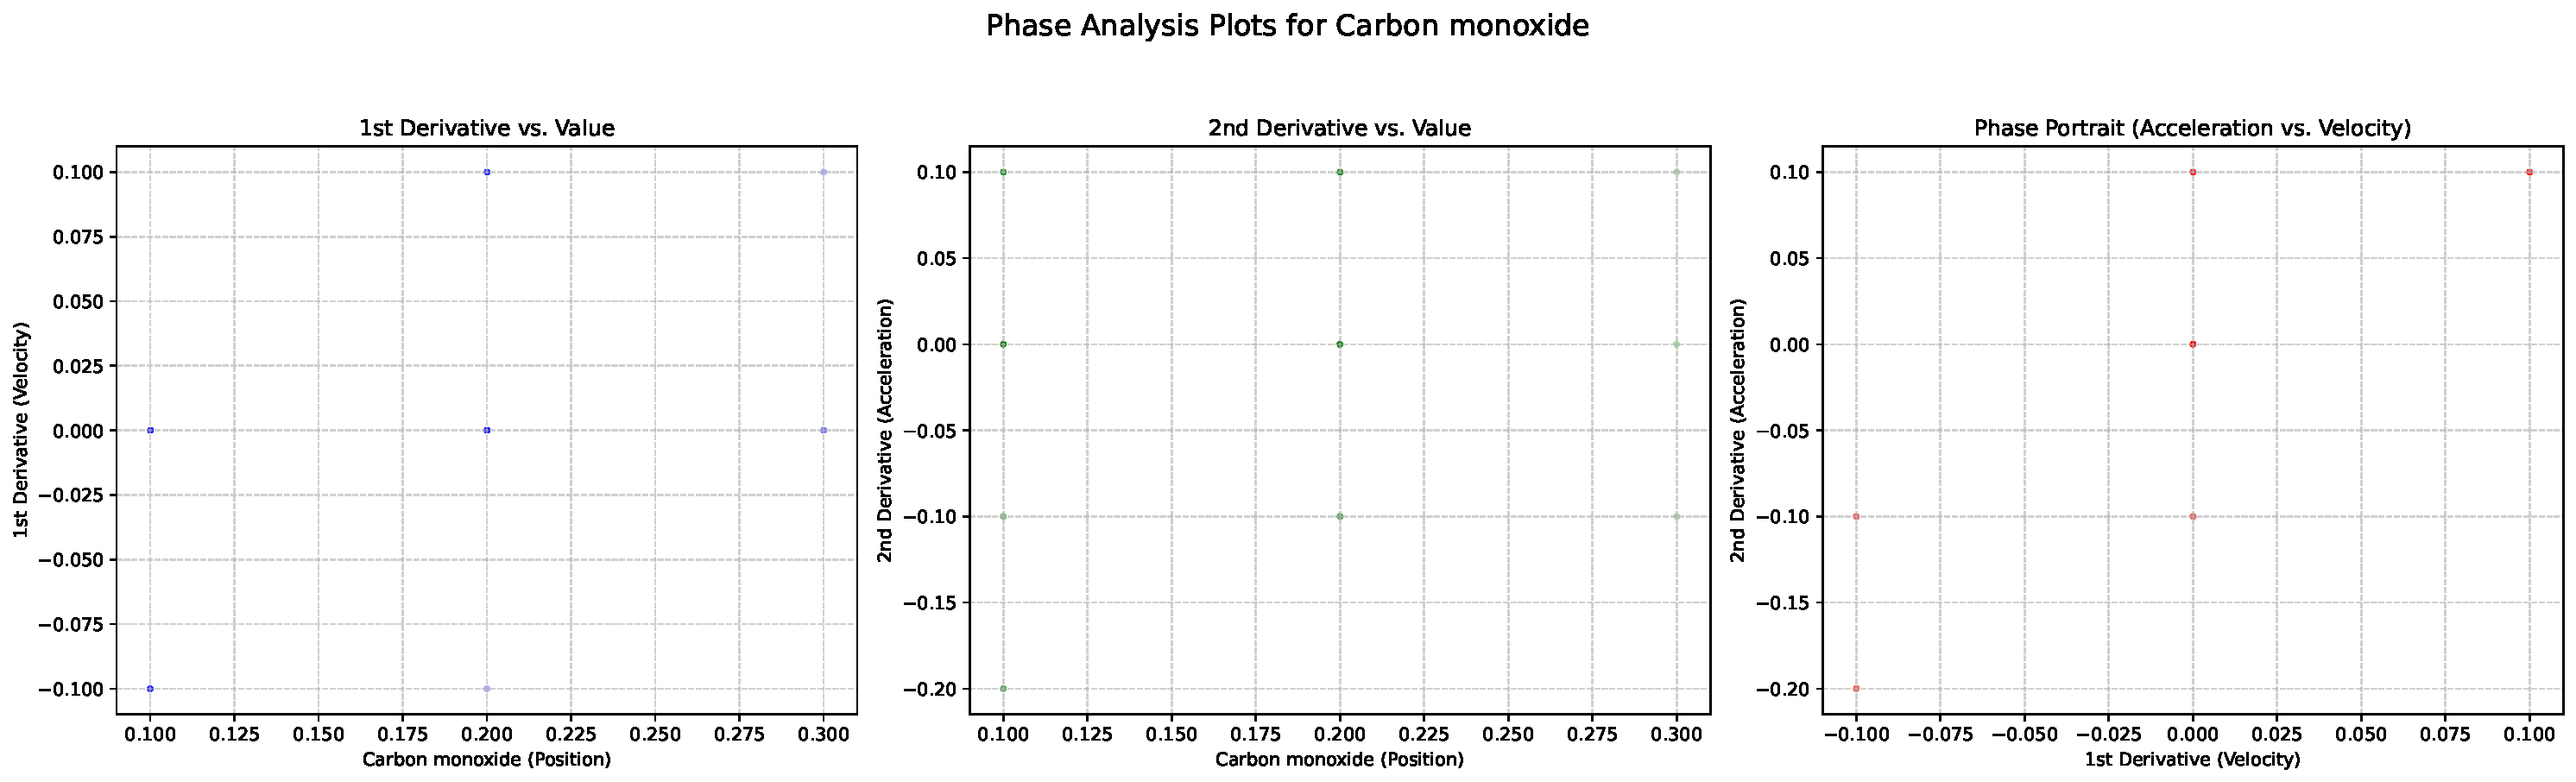
\includegraphics[width=0.8\textwidth]{../plots/khmelnytskyi_stats_plots/phase_analysis/phase_analysis_carbon_monoxide.pdf}
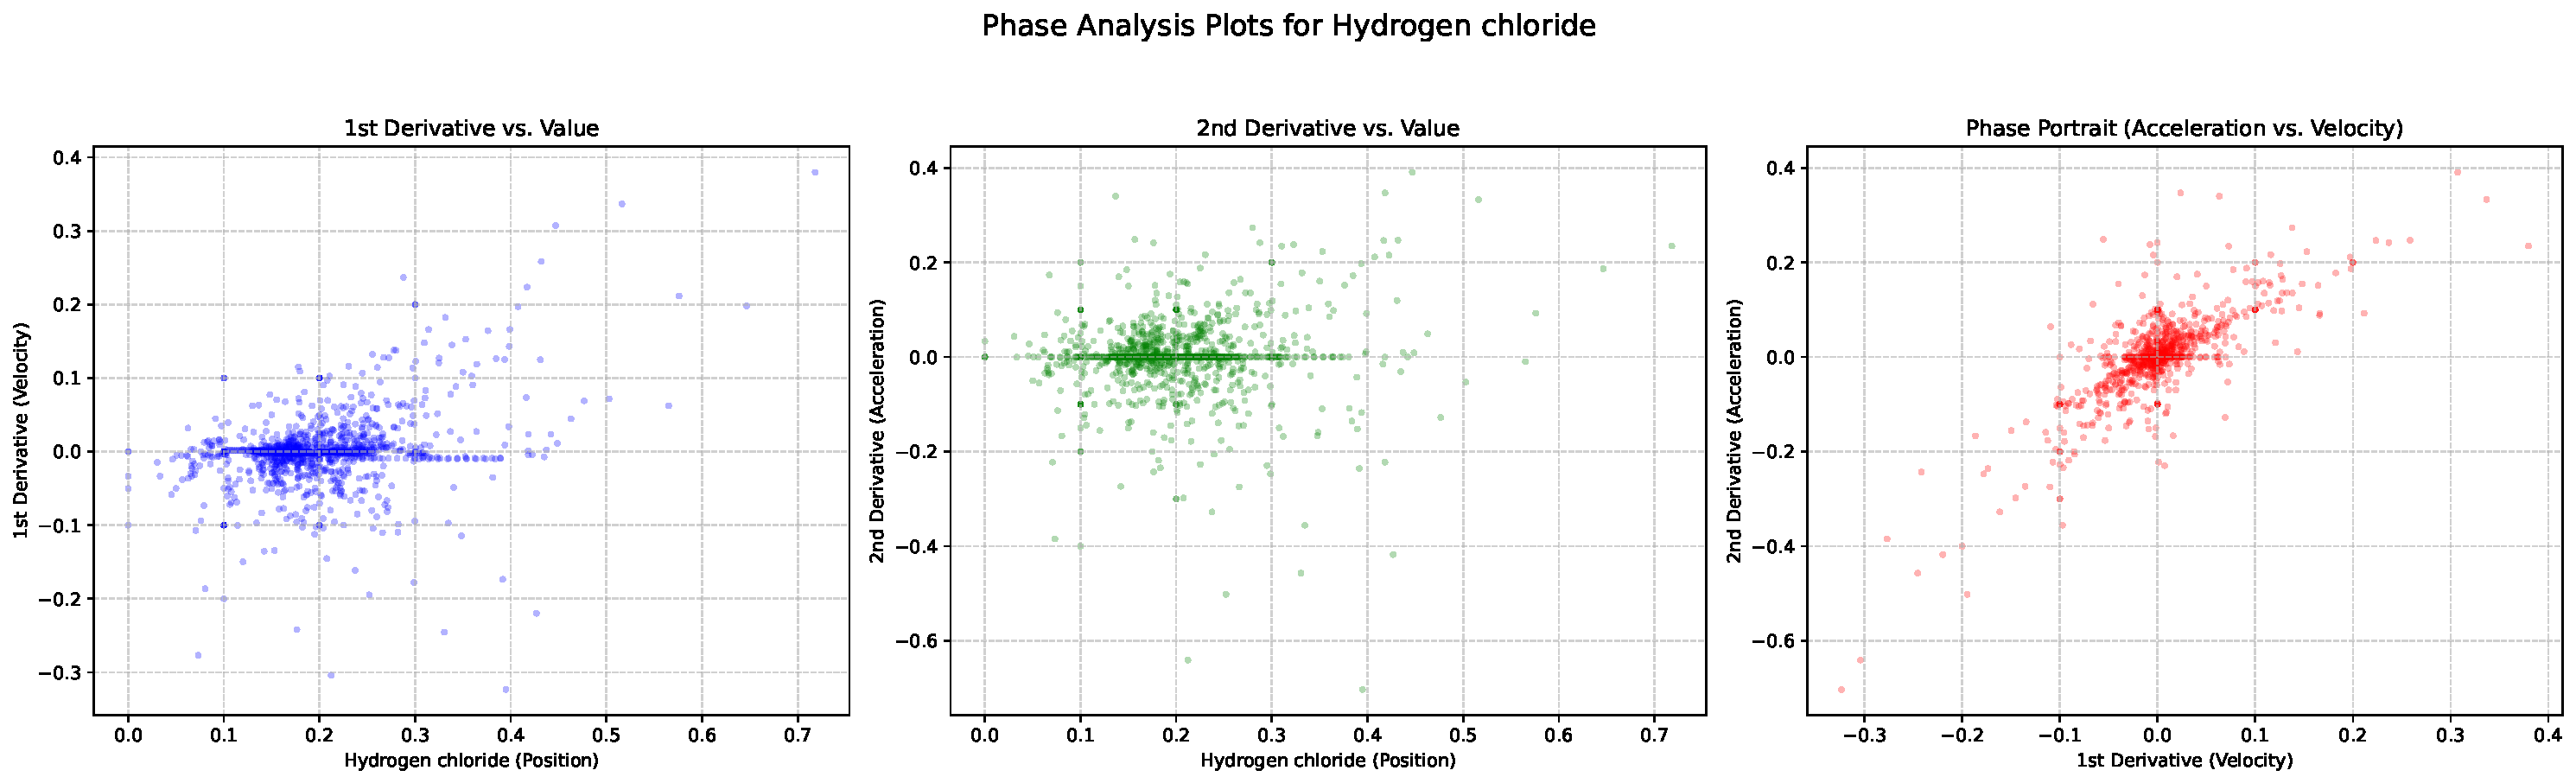
\includegraphics[width=0.8\textwidth]{../plots/khmelnytskyi_stats_plots/phase_analysis/phase_analysis_hydrogen_chloride.pdf}
\caption{Фазовий аналіз забруднюючих речовин в Хмельницькому. Графіки зображені лише для carbon monoxide та hydrogen chloride, але аналогічні графіки були побудувані і для інших забруднюючих речовин.}
\label{fig:phase_analysis}
\end{figure}

\subsection{Кореляційний аналіз}

Кореляційний аналіз дозволяє виявити залежності між різними забруднюючими
речовинами. Ми можемо обрахувати коефіцієнт кореляції Пірсона для кожної пари
забруднюючих речовин, щоб визначити, чи є між ними лінійна залежність. 
Код для обрахунку коефіцієнтів кореляції виглядає наступним чином:
\begin{minted}{python}
def perform_correlation_analysis(
    df, pollutant_columns, output_csv_dir: str = "csv"
) -> None:
    """
    Calculates the Pearson correlation matrix for the given pollutants
    and saves it to a CSV file.
    """
    
    print("Calculating pollutant correlation matrix...")
    if df.empty or not pollutant_columns:
        print("DataFrame is empty or no pollutant columns provided. Skipping correlation analysis.")
        return None

    try:
        # Select only pollutant columns for correlation
        pollutant_data = df[pollutant_columns]
        correlation_matrix = pollutant_data.corr(method='pearson')
    except Exception as e:
        print(f"Error calculating correlation matrix: {e}")
        return None

    output_path = Path(output_csv_dir)
    output_path.mkdir(parents=True, exist_ok=True) 
    correlation_file_path = output_path / "pollutant_correlation_matrix.csv"

    try:
        correlation_matrix.to_csv(correlation_file_path)
        print(f"Pollutant correlation matrix saved to: {correlation_file_path}")
    except Exception as e:
        print(f"Error saving correlation matrix to CSV: {e}")
        # Optionally return matrix even if saving fails, or return None
        # return correlation_matrix
        return None

    return correlation_matrix
\end{minted}

Ну і відповідно код для візуалізації кореляційної матриці:
\begin{minted}{python}
def plot_correlation_heatmap(correlation_matrix, output_dir="plots") -> None:
    """
    Plots a heatmap of the pollutant correlation matrix.

    Args:
        correlation_matrix (pd.DataFrame): The correlation matrix to plot.
        output_dir (str): Directory to save the heatmap PDF.
    """
    
    print("Generating correlation heatmap...")
    if correlation_matrix is None or correlation_matrix.empty:
        print("Correlation matrix is empty or None. Skipping heatmap plot.")
        return

    output_path = Path(output_dir)
    output_path.mkdir(parents=True, exist_ok=True)
    heatmap_file_path = output_path / "pollutant_correlation_heatmap.pdf"

    plt.figure(figsize=(max(10, len(correlation_matrix.columns) * 0.8), max(8, len(correlation_matrix.columns) * 0.7)))
    sns.heatmap(
        correlation_matrix,
        annot=True,          
        cmap='coolwarm',     
        fmt=".2f",          
        linewidths=.5,       
        vmin=-1, vmax=1,    
        cbar_kws={'label': 'Correlation Coefficient'}
    )
    plt.title('Correlation Matrix Heatmap', fontsize=16)
    plt.xticks(rotation=45, ha="right", fontsize=10)
    plt.yticks(rotation=0, fontsize=10)
    plt.tight_layout()

    try:
        plt.savefig(heatmap_file_path, dpi=300, format='pdf')
        print(f"Correlation heatmap saved to: {heatmap_file_path}")
    except Exception as e:
        print(f"Error saving correlation heatmap: {e}")
    plt.close()
\end{minted}

Результат кореляційного аналізу вийшов цікавий: див. Рисунок~\ref{fig:correlation_heatmap}.

\begin{figure}[H]
\centering
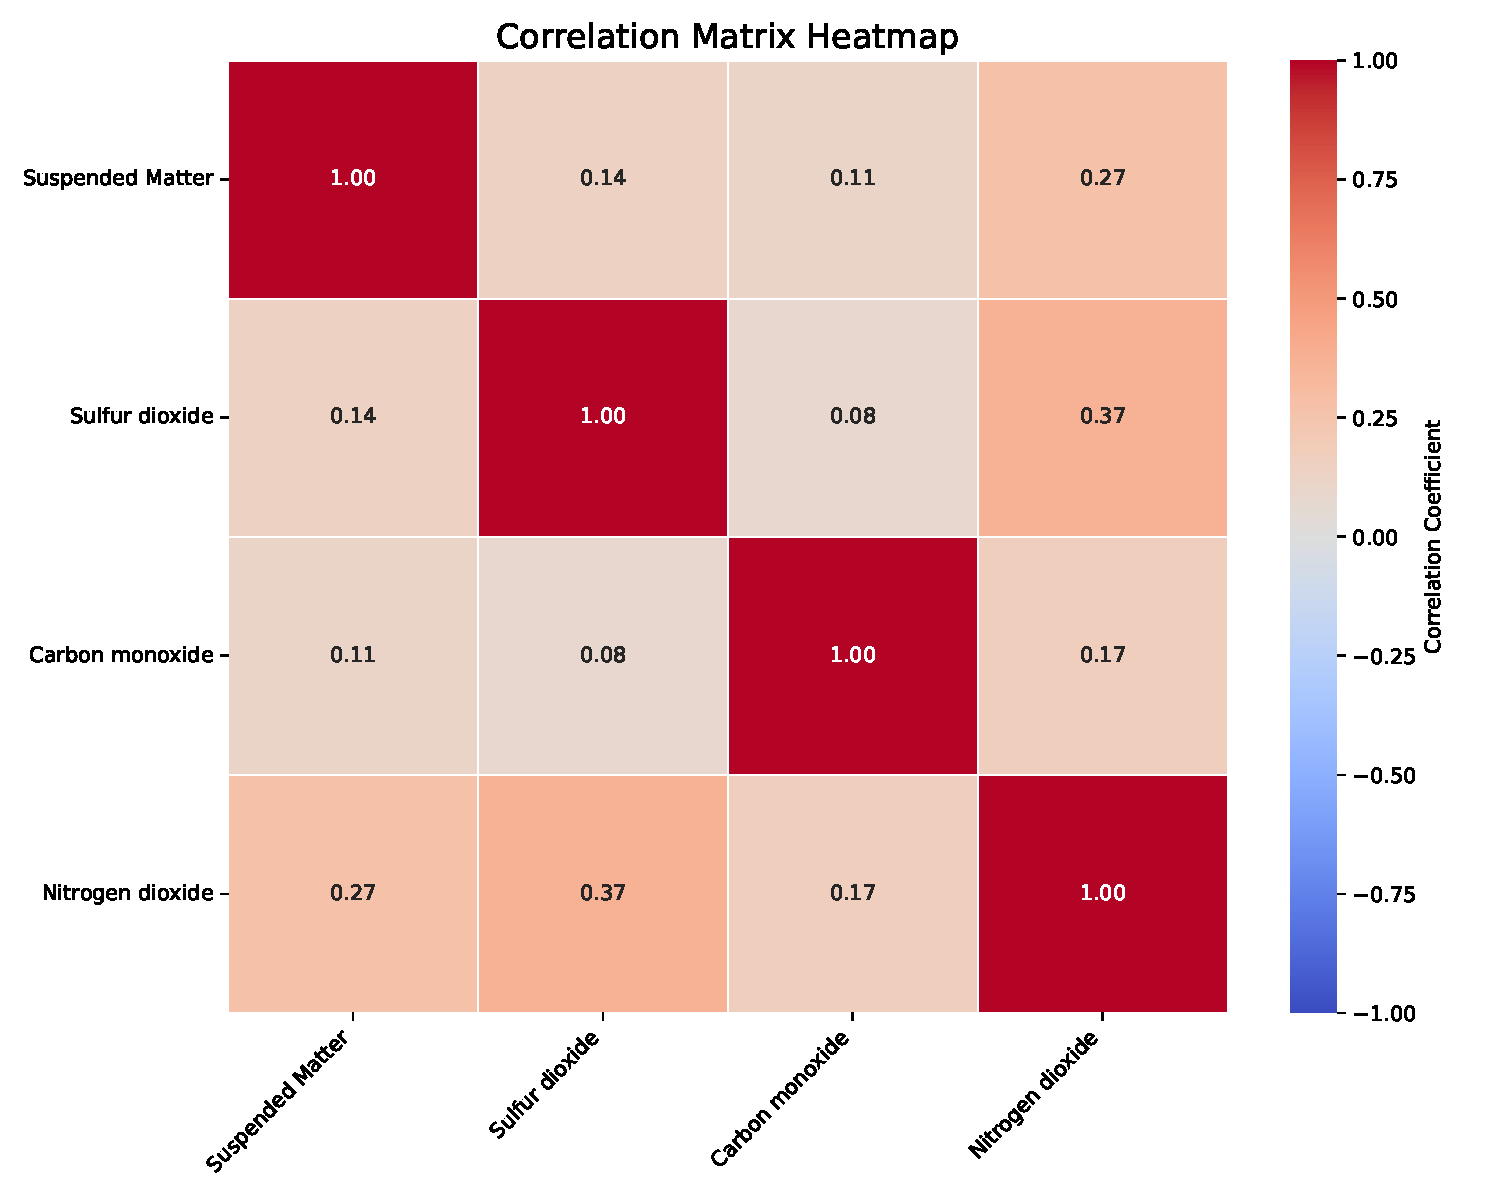
\includegraphics[width=\textwidth]{../plots/khmelnytskyi_stats_plots/correlation_analysis/pollutant_correlation_heatmap.pdf}
\caption{Кореляційна матриця забруднюючих речовин в Хмельницькому. Як бачимо,
найбільша кореляція спостерігається між formaldehyde та sulfur dioxide: а саме,
$0.51$, а також між phenol та formaldehyde, що дорівнює $0.5$. Це може свідчити
про те, що ці забруднюючі речовини мають спільні джерела викидів або взаємодіють
в атмосфері.}
\label{fig:correlation_heatmap}
\end{figure}

З цікавості, ми вирішили побудувати лінію регресії між 
формальдегідом та діоксидом сірки, щоб побачити, як змінюється рівень
формальдегіду в залежності від рівня діоксиду сірки. Маємо 
Рисунок~\ref{fig:regression_formaldehyde_sulfur_dioxide}.

\begin{figure}[H]
\centering
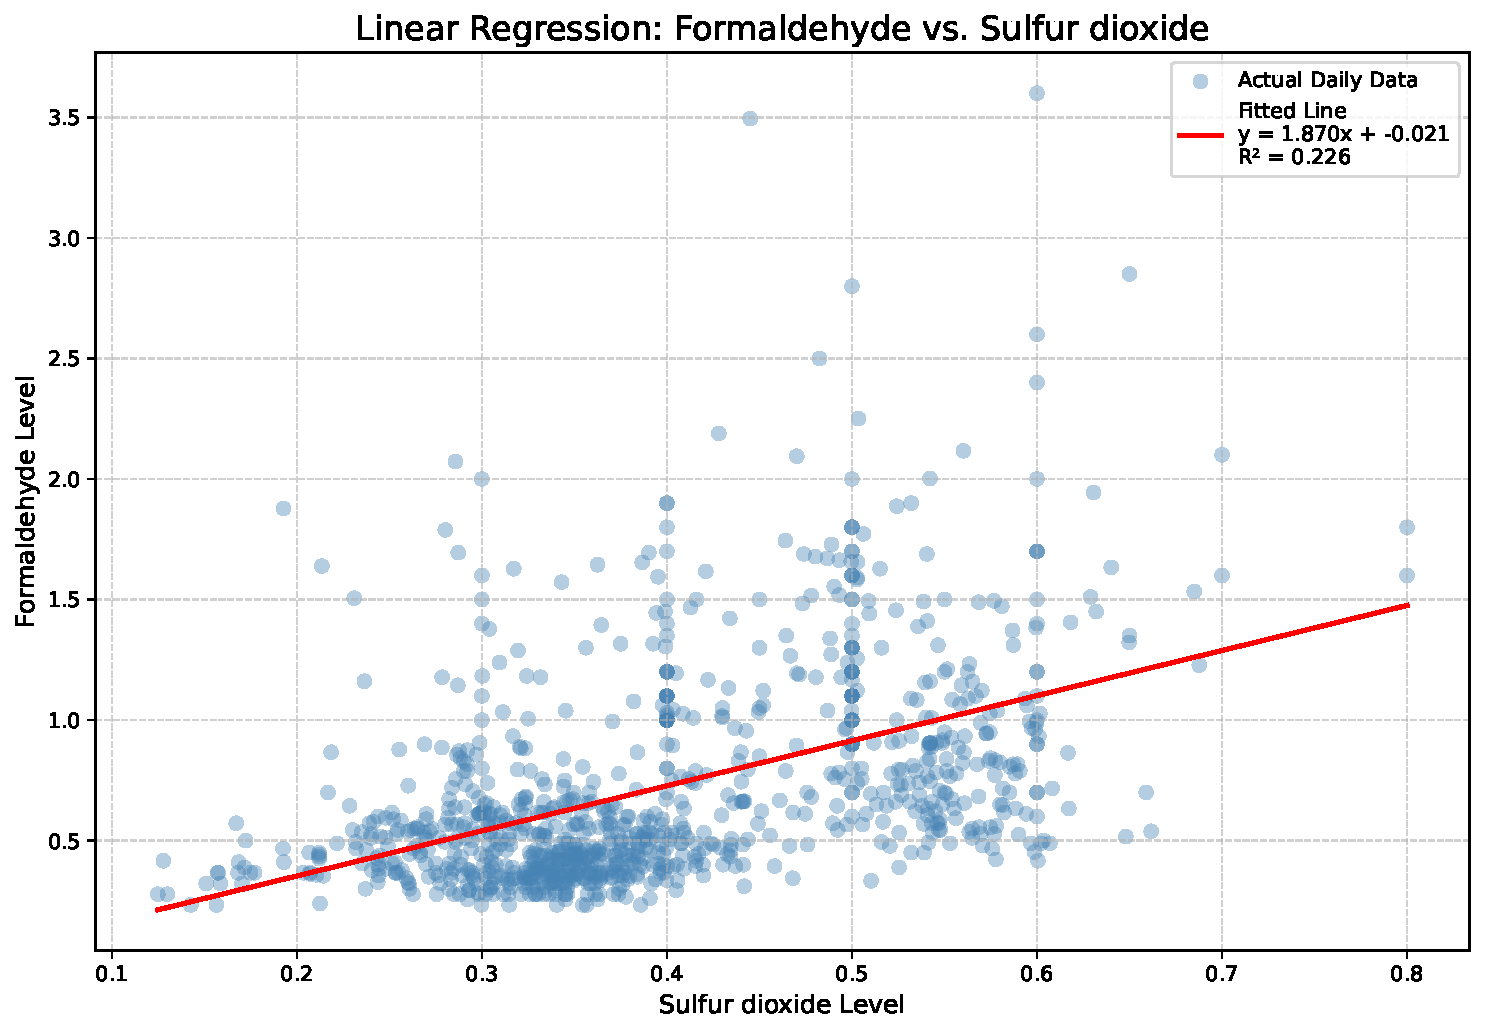
\includegraphics[width=0.8\textwidth]{../plots/khmelnytskyi_stats_plots/correlation_analysis/regression_formaldehyde_vs_sulfur_dioxide.pdf}
\caption{Лінія регресії $y(x) \approx 1.87x - 0.021$ між формальдегідом та
діоксидом сірки в Хмельницькому. Як бачимо, рівень формальдегіду зростає з
ростом рівня діоксиду сірки.}
\label{fig:regression_formaldehyde_sulfur_dioxide}
\end{figure}

\end{document}